\documentclass[twoside]{book}

% Packages required by doxygen
\usepackage{fixltx2e}
\usepackage{calc}
\usepackage{doxygen}
\usepackage[export]{adjustbox} % also loads graphicx
\usepackage{graphicx}
\usepackage[utf8]{inputenc}
\usepackage{makeidx}
\usepackage{multicol}
\usepackage{multirow}
\PassOptionsToPackage{warn}{textcomp}
\usepackage{textcomp}
\usepackage[nointegrals]{wasysym}
\usepackage[table]{xcolor}

% Font selection
\usepackage[T1]{fontenc}
\usepackage[scaled=.90]{helvet}
\usepackage{courier}
\usepackage{amssymb}
\usepackage{sectsty}
\renewcommand{\familydefault}{\sfdefault}
\allsectionsfont{%
  \fontseries{bc}\selectfont%
  \color{darkgray}%
}
\renewcommand{\DoxyLabelFont}{%
  \fontseries{bc}\selectfont%
  \color{darkgray}%
}
\newcommand{\+}{\discretionary{\mbox{\scriptsize$\hookleftarrow$}}{}{}}

% Page & text layout
\usepackage{geometry}
\geometry{%
  a4paper,%
  top=2.5cm,%
  bottom=2.5cm,%
  left=2.5cm,%
  right=2.5cm%
}
\tolerance=750
\hfuzz=15pt
\hbadness=750
\setlength{\emergencystretch}{15pt}
\setlength{\parindent}{0cm}
\setlength{\parskip}{3ex plus 2ex minus 2ex}
\makeatletter
\renewcommand{\paragraph}{%
  \@startsection{paragraph}{4}{0ex}{-1.0ex}{1.0ex}{%
    \normalfont\normalsize\bfseries\SS@parafont%
  }%
}
\renewcommand{\subparagraph}{%
  \@startsection{subparagraph}{5}{0ex}{-1.0ex}{1.0ex}{%
    \normalfont\normalsize\bfseries\SS@subparafont%
  }%
}
\makeatother

% Headers & footers
\usepackage{fancyhdr}
\pagestyle{fancyplain}
\fancyhead[LE]{\fancyplain{}{\bfseries\thepage}}
\fancyhead[CE]{\fancyplain{}{}}
\fancyhead[RE]{\fancyplain{}{\bfseries\leftmark}}
\fancyhead[LO]{\fancyplain{}{\bfseries\rightmark}}
\fancyhead[CO]{\fancyplain{}{}}
\fancyhead[RO]{\fancyplain{}{\bfseries\thepage}}
\fancyfoot[LE]{\fancyplain{}{}}
\fancyfoot[CE]{\fancyplain{}{}}
\fancyfoot[RE]{\fancyplain{}{\bfseries\scriptsize Generated by Doxygen }}
\fancyfoot[LO]{\fancyplain{}{\bfseries\scriptsize Generated by Doxygen }}
\fancyfoot[CO]{\fancyplain{}{}}
\fancyfoot[RO]{\fancyplain{}{}}
\renewcommand{\footrulewidth}{0.4pt}
\renewcommand{\chaptermark}[1]{%
  \markboth{#1}{}%
}
\renewcommand{\sectionmark}[1]{%
  \markright{\thesection\ #1}%
}

% Indices & bibliography
\usepackage{natbib}
\usepackage[titles]{tocloft}
\setcounter{tocdepth}{3}
\setcounter{secnumdepth}{5}
\makeindex

% Hyperlinks (required, but should be loaded last)
\usepackage{ifpdf}
\ifpdf
  \usepackage[pdftex,pagebackref=true]{hyperref}
\else
  \usepackage[ps2pdf,pagebackref=true]{hyperref}
\fi
\hypersetup{%
  colorlinks=true,%
  linkcolor=blue,%
  citecolor=blue,%
  unicode%
}

% Custom commands
\newcommand{\clearemptydoublepage}{%
  \newpage{\pagestyle{empty}\cleardoublepage}%
}

\usepackage{caption}
\captionsetup{labelsep=space,justification=centering,font={bf},singlelinecheck=off,skip=4pt,position=top}

%===== C O N T E N T S =====

\begin{document}

% Titlepage & ToC
\hypersetup{pageanchor=false,
             bookmarksnumbered=true,
             pdfencoding=unicode
            }
\pagenumbering{roman}
\begin{titlepage}
\vspace*{7cm}
\begin{center}%
{\Large U\+T\+Computer }\\
\vspace*{1cm}
{\large Generated by Doxygen 1.8.11}\\
\end{center}
\end{titlepage}
\clearemptydoublepage
\tableofcontents
\clearemptydoublepage
\pagenumbering{arabic}
\hypersetup{pageanchor=true}

%--- Begin generated contents ---
\chapter{Hierarchical Index}
\section{Class Hierarchy}
This inheritance list is sorted roughly, but not completely, alphabetically\+:\begin{DoxyCompactList}
\item \contentsline{section}{Expression\+Exception}{\pageref{class_expression_exception}}{}
\item \contentsline{section}{I\+Operand}{\pageref{class_i_operand}}{}
\begin{DoxyCompactList}
\item \contentsline{section}{I\+Literal}{\pageref{class_i_literal}}{}
\begin{DoxyCompactList}
\item \contentsline{section}{Complex\+Literal}{\pageref{class_complex_literal}}{}
\item \contentsline{section}{Expression\+Literal}{\pageref{class_expression_literal}}{}
\item \contentsline{section}{I\+Number\+Literal}{\pageref{class_i_number_literal}}{}
\begin{DoxyCompactList}
\item \contentsline{section}{Integer\+Literal}{\pageref{class_integer_literal}}{}
\item \contentsline{section}{Rational\+Literal}{\pageref{class_rational_literal}}{}
\item \contentsline{section}{Real\+Literal}{\pageref{class_real_literal}}{}
\end{DoxyCompactList}
\item \contentsline{section}{Program\+Literal}{\pageref{class_program_literal}}{}
\end{DoxyCompactList}
\item \contentsline{section}{I\+Operator}{\pageref{class_i_operator}}{}
\begin{DoxyCompactList}
\item \contentsline{section}{\$Op}{\pageref{class_0B_op}}{}
\item \contentsline{section}{And\+Op}{\pageref{class_and_op}}{}
\item \contentsline{section}{Clear\+Op}{\pageref{class_clear_op}}{}
\item \contentsline{section}{Den\+Op}{\pageref{class_den_op}}{}
\item \contentsline{section}{Different\+Op}{\pageref{class_different_op}}{}
\item \contentsline{section}{Div\+Ent\+Op}{\pageref{class_div_ent_op}}{}
\item \contentsline{section}{Div\+Op}{\pageref{class_div_op}}{}
\item \contentsline{section}{Drop\+Op}{\pageref{class_drop_op}}{}
\item \contentsline{section}{Dup\+Op}{\pageref{class_dup_op}}{}
\item \contentsline{section}{Equal\+Op}{\pageref{class_equal_op}}{}
\item \contentsline{section}{Eval\+Op}{\pageref{class_eval_op}}{}
\item \contentsline{section}{Ift\+Op}{\pageref{class_ift_op}}{}
\item \contentsline{section}{Im\+Op}{\pageref{class_im_op}}{}
\item \contentsline{section}{Inf\+Eq\+Op}{\pageref{class_inf_eq_op}}{}
\item \contentsline{section}{Inf\+Op}{\pageref{class_inf_op}}{}
\item \contentsline{section}{Minus\+Op}{\pageref{class_minus_op}}{}
\item \contentsline{section}{Modul\+Op}{\pageref{class_modul_op}}{}
\item \contentsline{section}{Multi\+Op}{\pageref{class_multi_op}}{}
\item \contentsline{section}{Neg\+Op}{\pageref{class_neg_op}}{}
\item \contentsline{section}{Not\+Op}{\pageref{class_not_op}}{}
\item \contentsline{section}{Num\+Op}{\pageref{class_num_op}}{}
\item \contentsline{section}{Or\+Op}{\pageref{class_or_op}}{}
\item \contentsline{section}{Plus\+Op}{\pageref{class_plus_op}}{}
\item \contentsline{section}{Redo\+Op}{\pageref{class_redo_op}}{}
\item \contentsline{section}{Re\+Op}{\pageref{class_re_op}}{}
\item \contentsline{section}{Sup\+Eq\+Op}{\pageref{class_sup_eq_op}}{}
\item \contentsline{section}{Sup\+Op}{\pageref{class_sup_op}}{}
\item \contentsline{section}{Swap\+Op}{\pageref{class_swap_op}}{}
\item \contentsline{section}{Undo\+Op}{\pageref{class_undo_op}}{}
\end{DoxyCompactList}
\end{DoxyCompactList}
\item \contentsline{section}{Literal\+Factory}{\pageref{class_literal_factory}}{}
\item \contentsline{section}{Operator\+Exception}{\pageref{class_operator_exception}}{}
\item Q\+Object\begin{DoxyCompactList}
\item \contentsline{section}{Controller}{\pageref{class_controller}}{}
\end{DoxyCompactList}
\item \contentsline{section}{qt\+\_\+meta\+\_\+stringdata\+\_\+\+Controller\+\_\+t}{\pageref{structqt__meta__stringdata___controller__t}}{}
\item \contentsline{section}{qt\+\_\+meta\+\_\+stringdata\+\_\+\+Q\+Computer\+\_\+t}{\pageref{structqt__meta__stringdata___q_computer__t}}{}
\item Q\+Widget\begin{DoxyCompactList}
\item \contentsline{section}{Q\+Computer}{\pageref{class_q_computer}}{}
\end{DoxyCompactList}
\item \contentsline{section}{Stack}{\pageref{class_stack}}{}
\item \contentsline{section}{Stack\+Memento}{\pageref{class_stack_memento}}{}
\end{DoxyCompactList}

\chapter{Class Index}
\section{Class List}
Here are the classes, structs, unions and interfaces with brief descriptions\+:\begin{DoxyCompactList}
\item\contentsline{section}{\hyperlink{class_0B_op}{\$\+Op} }{\pageref{class_0B_op}}{}
\item\contentsline{section}{\hyperlink{class_and_op}{And\+Op} }{\pageref{class_and_op}}{}
\item\contentsline{section}{\hyperlink{class_clear_op}{Clear\+Op} }{\pageref{class_clear_op}}{}
\item\contentsline{section}{\hyperlink{class_complex_literal}{Complex\+Literal} }{\pageref{class_complex_literal}}{}
\item\contentsline{section}{\hyperlink{class_controller}{Controller} \\*Gere les variables, les programmes, le parser, les etats de la pile et les erreurs }{\pageref{class_controller}}{}
\item\contentsline{section}{\hyperlink{class_den_op}{Den\+Op} }{\pageref{class_den_op}}{}
\item\contentsline{section}{\hyperlink{class_different_op}{Different\+Op} }{\pageref{class_different_op}}{}
\item\contentsline{section}{\hyperlink{class_div_ent_op}{Div\+Ent\+Op} \\*Execute le deuxieme element division entiere par le premier de lap ile }{\pageref{class_div_ent_op}}{}
\item\contentsline{section}{\hyperlink{class_div_op}{Div\+Op} \\*Execute le deuxieme element divise par le premier de la pile }{\pageref{class_div_op}}{}
\item\contentsline{section}{\hyperlink{class_drop_op}{Drop\+Op} }{\pageref{class_drop_op}}{}
\item\contentsline{section}{\hyperlink{class_dup_op}{Dup\+Op} }{\pageref{class_dup_op}}{}
\item\contentsline{section}{\hyperlink{class_equal_op}{Equal\+Op} }{\pageref{class_equal_op}}{}
\item\contentsline{section}{\hyperlink{class_eval_op}{Eval\+Op} }{\pageref{class_eval_op}}{}
\item\contentsline{section}{\hyperlink{class_expression_exception}{Expression\+Exception} }{\pageref{class_expression_exception}}{}
\item\contentsline{section}{\hyperlink{class_expression_literal}{Expression\+Literal} }{\pageref{class_expression_literal}}{}
\item\contentsline{section}{\hyperlink{class_ift_op}{Ift\+Op} }{\pageref{class_ift_op}}{}
\item\contentsline{section}{\hyperlink{class_i_literal}{I\+Literal} }{\pageref{class_i_literal}}{}
\item\contentsline{section}{\hyperlink{class_im_op}{Im\+Op} }{\pageref{class_im_op}}{}
\item\contentsline{section}{\hyperlink{class_inf_eq_op}{Inf\+Eq\+Op} }{\pageref{class_inf_eq_op}}{}
\item\contentsline{section}{\hyperlink{class_inf_op}{Inf\+Op} }{\pageref{class_inf_op}}{}
\item\contentsline{section}{\hyperlink{class_integer_literal}{Integer\+Literal} }{\pageref{class_integer_literal}}{}
\item\contentsline{section}{\hyperlink{class_i_number_literal}{I\+Number\+Literal} }{\pageref{class_i_number_literal}}{}
\item\contentsline{section}{\hyperlink{class_i_operand}{I\+Operand} }{\pageref{class_i_operand}}{}
\item\contentsline{section}{\hyperlink{class_i_operator}{I\+Operator} \\*Classe abstraite dont chaque operateur heritera }{\pageref{class_i_operator}}{}
\item\contentsline{section}{\hyperlink{class_literal_factory}{Literal\+Factory} }{\pageref{class_literal_factory}}{}
\item\contentsline{section}{\hyperlink{class_minus_op}{Minus\+Op} \\*Execute le deuxi�me element -\/ le premier }{\pageref{class_minus_op}}{}
\item\contentsline{section}{\hyperlink{class_modul_op}{Modul\+Op} \\*Modulo du premier element par le deuxieme }{\pageref{class_modul_op}}{}
\item\contentsline{section}{\hyperlink{class_multi_op}{Multi\+Op} \\*Execute \textquotesingle{}$\ast$\textquotesingle{} sur les deux premiers element de la pile }{\pageref{class_multi_op}}{}
\item\contentsline{section}{\hyperlink{class_neg_op}{Neg\+Op} \\*Permet de changer le signe d\textquotesingle{}une valeur }{\pageref{class_neg_op}}{}
\item\contentsline{section}{\hyperlink{class_not_op}{Not\+Op} }{\pageref{class_not_op}}{}
\item\contentsline{section}{\hyperlink{class_num_op}{Num\+Op} }{\pageref{class_num_op}}{}
\item\contentsline{section}{\hyperlink{class_operator_exception}{Operator\+Exception} }{\pageref{class_operator_exception}}{}
\item\contentsline{section}{\hyperlink{class_or_op}{Or\+Op} }{\pageref{class_or_op}}{}
\item\contentsline{section}{\hyperlink{class_plus_op}{Plus\+Op} \\*Execute \textquotesingle{}+\textquotesingle{} sur les deux premiers element de la pile }{\pageref{class_plus_op}}{}
\item\contentsline{section}{\hyperlink{class_program_literal}{Program\+Literal} }{\pageref{class_program_literal}}{}
\item\contentsline{section}{\hyperlink{class_q_computer}{Q\+Computer} }{\pageref{class_q_computer}}{}
\item\contentsline{section}{\hyperlink{structqt__meta__stringdata___controller__t}{qt\+\_\+meta\+\_\+stringdata\+\_\+\+Controller\+\_\+t} }{\pageref{structqt__meta__stringdata___controller__t}}{}
\item\contentsline{section}{\hyperlink{structqt__meta__stringdata___q_computer__t}{qt\+\_\+meta\+\_\+stringdata\+\_\+\+Q\+Computer\+\_\+t} }{\pageref{structqt__meta__stringdata___q_computer__t}}{}
\item\contentsline{section}{\hyperlink{class_rational_literal}{Rational\+Literal} }{\pageref{class_rational_literal}}{}
\item\contentsline{section}{\hyperlink{class_real_literal}{Real\+Literal} }{\pageref{class_real_literal}}{}
\item\contentsline{section}{\hyperlink{class_redo_op}{Redo\+Op} }{\pageref{class_redo_op}}{}
\item\contentsline{section}{\hyperlink{class_re_op}{Re\+Op} }{\pageref{class_re_op}}{}
\item\contentsline{section}{\hyperlink{class_stack}{Stack} }{\pageref{class_stack}}{}
\item\contentsline{section}{\hyperlink{class_stack_memento}{Stack\+Memento} }{\pageref{class_stack_memento}}{}
\item\contentsline{section}{\hyperlink{class_sup_eq_op}{Sup\+Eq\+Op} }{\pageref{class_sup_eq_op}}{}
\item\contentsline{section}{\hyperlink{class_sup_op}{Sup\+Op} }{\pageref{class_sup_op}}{}
\item\contentsline{section}{\hyperlink{class_swap_op}{Swap\+Op} }{\pageref{class_swap_op}}{}
\item\contentsline{section}{\hyperlink{class_undo_op}{Undo\+Op} }{\pageref{class_undo_op}}{}
\end{DoxyCompactList}

\chapter{File Index}
\section{File List}
Here is a list of all documented files with brief descriptions\+:\begin{DoxyCompactList}
\item\contentsline{section}{D\+:/\+Cours/\+U\+T\+C/\+P16/\+L\+O21/\+U\+T\+Computer/\+U\+T\+Computer/\hyperlink{_controller_8h}{Controller.\+h} \\*Contient le controller de la calculette }{\pageref{_controller_8h}}{}
\item\contentsline{section}{D\+:/\+Cours/\+U\+T\+C/\+P16/\+L\+O21/\+U\+T\+Computer/\+U\+T\+Computer/{\bfseries Expression\+Parser.\+h} }{\pageref{_expression_parser_8h}}{}
\item\contentsline{section}{D\+:/\+Cours/\+U\+T\+C/\+P16/\+L\+O21/\+U\+T\+Computer/\+U\+T\+Computer/{\bfseries Literal.\+h} }{\pageref{_literal_8h}}{}
\item\contentsline{section}{D\+:/\+Cours/\+U\+T\+C/\+P16/\+L\+O21/\+U\+T\+Computer/\+U\+T\+Computer/{\bfseries Literal\+Factory.\+h} }{\pageref{_literal_factory_8h}}{}
\item\contentsline{section}{D\+:/\+Cours/\+U\+T\+C/\+P16/\+L\+O21/\+U\+T\+Computer/\+U\+T\+Computer/\hyperlink{_operator_8h}{Operator.\+h} \\*Contient tous les operateurs possibles dans la calculette }{\pageref{_operator_8h}}{}
\item\contentsline{section}{D\+:/\+Cours/\+U\+T\+C/\+P16/\+L\+O21/\+U\+T\+Computer/\+U\+T\+Computer/{\bfseries Operator\+Exception.\+h} }{\pageref{_operator_exception_8h}}{}
\item\contentsline{section}{D\+:/\+Cours/\+U\+T\+C/\+P16/\+L\+O21/\+U\+T\+Computer/\+U\+T\+Computer/{\bfseries qcomputer.\+h} }{\pageref{qcomputer_8h}}{}
\item\contentsline{section}{D\+:/\+Cours/\+U\+T\+C/\+P16/\+L\+O21/\+U\+T\+Computer/\+U\+T\+Computer/{\bfseries Stack.\+h} }{\pageref{_stack_8h}}{}
\item\contentsline{section}{D\+:/\+Cours/\+U\+T\+C/\+P16/\+L\+O21/\+U\+T\+Computer/\+U\+T\+Computer/{\bfseries Stack\+Memento.\+h} }{\pageref{_stack_memento_8h}}{}
\item\contentsline{section}{D\+:/\+Cours/\+U\+T\+C/\+P16/\+L\+O21/\+U\+T\+Computer/\+U\+T\+Computer/{\bfseries test.\+h} }{\pageref{test_8h}}{}
\end{DoxyCompactList}

\chapter{Class Documentation}
\hypertarget{class_0B_op}{}\section{\$Op Class Reference}
\label{class_0B_op}\index{\$\+Op@{\$\+Op}}
Inheritance diagram for \$Op\+:\begin{figure}[H]
\begin{center}
\leavevmode
\includegraphics[height=3.000000cm]{class_0B_op}
\end{center}
\end{figure}
\subsection*{Public Member Functions}
\begin{DoxyCompactItemize}
\item 
void \hyperlink{class_0B_op_aee5cf8ea506c3bd12523631be240095f}{operator()} (\hyperlink{class_stack}{Stack} $\ast$s)
\begin{DoxyCompactList}\small\item\em Methode virtuel redefini par chaque operator pour definir la fonction de l\textquotesingle{}operateur. \end{DoxyCompactList}\end{DoxyCompactItemize}


\subsection{Member Function Documentation}
\index{\$\+Op@{\$\+Op}!operator()@{operator()}}
\index{operator()@{operator()}!\$\+Op@{\$\+Op}}
\subsubsection[{\texorpdfstring{operator()(\+Stack $\ast$s)}{operator()(Stack *s)}}]{\setlength{\rightskip}{0pt plus 5cm}void \$Op\+::operator() (
\begin{DoxyParamCaption}
\item[{{\bf Stack} $\ast$}]{s}
\end{DoxyParamCaption}
)\hspace{0.3cm}{\ttfamily [virtual]}}\hypertarget{class_0B_op_aee5cf8ea506c3bd12523631be240095f}{}\label{class_0B_op_aee5cf8ea506c3bd12523631be240095f}


Methode virtuel redefini par chaque operator pour definir la fonction de l\textquotesingle{}operateur. 

Methode principale de l\textquotesingle{}operateur \+: execute une action definie pour chaque operateur


\begin{DoxyParams}{Parameters}
{\em s} & \+: Reference sur la stack pour executer l\textquotesingle{}operateur \\
\hline
\end{DoxyParams}


Implements \hyperlink{class_i_operator_ab93ebb15195290da26e2f3e626f6f25e}{I\+Operator}.



The documentation for this class was generated from the following files\+:\begin{DoxyCompactItemize}
\item 
D\+:/\+Cours/\+U\+T\+C/\+P16/\+L\+O21/\+U\+T\+Computer/\+U\+T\+Computer/\hyperlink{_operator_8h}{Operator.\+h}\item 
D\+:/\+Cours/\+U\+T\+C/\+P16/\+L\+O21/\+U\+T\+Computer/\+U\+T\+Computer/Operator.\+cpp\end{DoxyCompactItemize}

\hypertarget{class_and_op}{}\section{And\+Op Class Reference}
\label{class_and_op}\index{And\+Op@{And\+Op}}
Inheritance diagram for And\+Op\+:\begin{figure}[H]
\begin{center}
\leavevmode
\includegraphics[height=3.000000cm]{class_and_op}
\end{center}
\end{figure}
\subsection*{Public Member Functions}
\begin{DoxyCompactItemize}
\item 
void \hyperlink{class_and_op_a9d22089abf7a345221af90d050115f09}{operator()} (\hyperlink{class_stack}{Stack} $\ast$s)
\begin{DoxyCompactList}\small\item\em Methode virtuel redefini par chaque operator pour definir la fonction de l\textquotesingle{}operateur. \end{DoxyCompactList}\end{DoxyCompactItemize}


\subsection{Member Function Documentation}
\index{And\+Op@{And\+Op}!operator()@{operator()}}
\index{operator()@{operator()}!And\+Op@{And\+Op}}
\subsubsection[{\texorpdfstring{operator()(\+Stack $\ast$s)}{operator()(Stack *s)}}]{\setlength{\rightskip}{0pt plus 5cm}void And\+Op\+::operator() (
\begin{DoxyParamCaption}
\item[{{\bf Stack} $\ast$}]{s}
\end{DoxyParamCaption}
)\hspace{0.3cm}{\ttfamily [virtual]}}\hypertarget{class_and_op_a9d22089abf7a345221af90d050115f09}{}\label{class_and_op_a9d22089abf7a345221af90d050115f09}


Methode virtuel redefini par chaque operator pour definir la fonction de l\textquotesingle{}operateur. 

Methode principale de l\textquotesingle{}operateur \+: execute une action definie pour chaque operateur


\begin{DoxyParams}{Parameters}
{\em s} & \+: Reference sur la stack pour executer l\textquotesingle{}operateur \\
\hline
\end{DoxyParams}


Implements \hyperlink{class_i_operator_ab93ebb15195290da26e2f3e626f6f25e}{I\+Operator}.



The documentation for this class was generated from the following files\+:\begin{DoxyCompactItemize}
\item 
D\+:/\+Cours/\+U\+T\+C/\+P16/\+L\+O21/\+U\+T\+Computer/\+U\+T\+Computer/\hyperlink{_operator_8h}{Operator.\+h}\item 
D\+:/\+Cours/\+U\+T\+C/\+P16/\+L\+O21/\+U\+T\+Computer/\+U\+T\+Computer/Operator.\+cpp\end{DoxyCompactItemize}

\hypertarget{class_clear_op}{}\section{Clear\+Op Class Reference}
\label{class_clear_op}\index{Clear\+Op@{Clear\+Op}}
Inheritance diagram for Clear\+Op\+:\begin{figure}[H]
\begin{center}
\leavevmode
\includegraphics[height=3.000000cm]{class_clear_op}
\end{center}
\end{figure}
\subsection*{Public Member Functions}
\begin{DoxyCompactItemize}
\item 
void \hyperlink{class_clear_op_aa1175887332f472c80576559e38c105e}{operator()} (\hyperlink{class_stack}{Stack} $\ast$s)
\begin{DoxyCompactList}\small\item\em Methode virtuel redefini par chaque operator pour definir la fonction de l\textquotesingle{}operateur. \end{DoxyCompactList}\end{DoxyCompactItemize}


\subsection{Member Function Documentation}
\index{Clear\+Op@{Clear\+Op}!operator()@{operator()}}
\index{operator()@{operator()}!Clear\+Op@{Clear\+Op}}
\subsubsection[{\texorpdfstring{operator()(\+Stack $\ast$s)}{operator()(Stack *s)}}]{\setlength{\rightskip}{0pt plus 5cm}void Clear\+Op\+::operator() (
\begin{DoxyParamCaption}
\item[{{\bf Stack} $\ast$}]{s}
\end{DoxyParamCaption}
)\hspace{0.3cm}{\ttfamily [virtual]}}\hypertarget{class_clear_op_aa1175887332f472c80576559e38c105e}{}\label{class_clear_op_aa1175887332f472c80576559e38c105e}


Methode virtuel redefini par chaque operator pour definir la fonction de l\textquotesingle{}operateur. 

Methode principale de l\textquotesingle{}operateur \+: execute une action definie pour chaque operateur


\begin{DoxyParams}{Parameters}
{\em s} & \+: Reference sur la stack pour executer l\textquotesingle{}operateur \\
\hline
\end{DoxyParams}


Implements \hyperlink{class_i_operator_ab93ebb15195290da26e2f3e626f6f25e}{I\+Operator}.



The documentation for this class was generated from the following files\+:\begin{DoxyCompactItemize}
\item 
D\+:/\+Cours/\+U\+T\+C/\+P16/\+L\+O21/\+U\+T\+Computer/\+U\+T\+Computer/\hyperlink{_operator_8h}{Operator.\+h}\item 
D\+:/\+Cours/\+U\+T\+C/\+P16/\+L\+O21/\+U\+T\+Computer/\+U\+T\+Computer/Operator.\+cpp\end{DoxyCompactItemize}

\hypertarget{class_complex_literal}{}\section{Complex\+Literal Class Reference}
\label{class_complex_literal}\index{Complex\+Literal@{Complex\+Literal}}
Inheritance diagram for Complex\+Literal\+:\begin{figure}[H]
\begin{center}
\leavevmode
\includegraphics[height=3.000000cm]{class_complex_literal}
\end{center}
\end{figure}
\subsection*{Public Member Functions}
\begin{DoxyCompactItemize}
\item 
{\bfseries Complex\+Literal} (\hyperlink{class_i_number_literal}{I\+Number\+Literal} $\ast$r=new \hyperlink{class_integer_literal}{Integer\+Literal}(0), \hyperlink{class_i_number_literal}{I\+Number\+Literal} $\ast$i=new \hyperlink{class_integer_literal}{Integer\+Literal}(0))\hypertarget{class_complex_literal_a49f6f9936ffbbcad5b1aa5b99f0202f9}{}\label{class_complex_literal_a49f6f9936ffbbcad5b1aa5b99f0202f9}

\item 
\hyperlink{class_i_literal}{I\+Literal} $\ast$ {\bfseries clone} () const \hypertarget{class_complex_literal_ad76d4572dafd9dcd4e82dcd20b0d1b57}{}\label{class_complex_literal_ad76d4572dafd9dcd4e82dcd20b0d1b57}

\item 
std\+::string {\bfseries to\+String} () const \hypertarget{class_complex_literal_aa1a06301b9dece737217a1684187b711}{}\label{class_complex_literal_aa1a06301b9dece737217a1684187b711}

\item 
\hyperlink{class_i_number_literal}{I\+Number\+Literal} \& {\bfseries Re} () const \hypertarget{class_complex_literal_a3ddf29d8fb18f80b6081cace78013bb3}{}\label{class_complex_literal_a3ddf29d8fb18f80b6081cace78013bb3}

\item 
\hyperlink{class_i_number_literal}{I\+Number\+Literal} \& {\bfseries Im} () const \hypertarget{class_complex_literal_a4fafc3f6a30fcb332ed7fbdcf3241881}{}\label{class_complex_literal_a4fafc3f6a30fcb332ed7fbdcf3241881}

\item 
Type {\bfseries get\+Type\+Real} () const \hypertarget{class_complex_literal_abf18f83dd1ee3173aa9fbcb40a71aed1}{}\label{class_complex_literal_abf18f83dd1ee3173aa9fbcb40a71aed1}

\item 
Type {\bfseries get\+Type\+Im} () const \hypertarget{class_complex_literal_a8e1880f4100f287d9e454ea5114ff040}{}\label{class_complex_literal_a8e1880f4100f287d9e454ea5114ff040}

\end{DoxyCompactItemize}
\subsection*{Private Attributes}
\begin{DoxyCompactItemize}
\item 
\hyperlink{class_i_number_literal}{I\+Number\+Literal} $\ast$ {\bfseries real}\hypertarget{class_complex_literal_a6c1c1abf5cdfb4a8ab997d81c816c1db}{}\label{class_complex_literal_a6c1c1abf5cdfb4a8ab997d81c816c1db}

\item 
\hyperlink{class_i_number_literal}{I\+Number\+Literal} $\ast$ {\bfseries imaginary}\hypertarget{class_complex_literal_aebcff0eab4cea0fe08e87c8cf76ed528}{}\label{class_complex_literal_aebcff0eab4cea0fe08e87c8cf76ed528}

\end{DoxyCompactItemize}


The documentation for this class was generated from the following file\+:\begin{DoxyCompactItemize}
\item 
D\+:/\+Cours/\+U\+T\+C/\+P16/\+L\+O21/\+U\+T\+Computer/\+U\+T\+Computer/Literal.\+h\end{DoxyCompactItemize}

\hypertarget{class_controller}{}\section{Controller Class Reference}
\label{class_controller}\index{Controller@{Controller}}


Gere les variables, les programmes, le parser, les etats de la pile et les erreurs.  




{\ttfamily \#include $<$Controller.\+h$>$}

Inheritance diagram for Controller\+:\begin{figure}[H]
\begin{center}
\leavevmode
\includegraphics[height=2.000000cm]{class_controller}
\end{center}
\end{figure}
\subsection*{Signals}
\begin{DoxyCompactItemize}
\item 
void \hyperlink{class_controller_a783956d7ffd422c814c8d62926c38f5c}{change\+State} ()
\begin{DoxyCompactList}\small\item\em Signal pour prevenir qu\textquotesingle{}il y a un changement de l\textquotesingle{}etat de la pile. \end{DoxyCompactList}\item 
void \hyperlink{class_controller_a82364c4f38974097562fb51658a0fe57}{show\+Error} (std\+::string error)
\begin{DoxyCompactList}\small\item\em Signal pour prevenir qu\textquotesingle{}il y a une erreur a afficher. \end{DoxyCompactList}\end{DoxyCompactItemize}
\subsection*{Public Member Functions}
\begin{DoxyCompactItemize}
\item 
void \hyperlink{class_controller_a0d63fc78835ccac86a76fd8ced6e0493}{command} (const std\+::string \&str)
\begin{DoxyCompactList}\small\item\em Execute des fonctions selon la string. \end{DoxyCompactList}\item 
void \hyperlink{class_controller_a61a7e0cd9d6c886c6e3dda8152a4f97c}{execute} (std\+::string op)
\begin{DoxyCompactList}\small\item\em Execute l\textquotesingle{}operateur envoye en param. \end{DoxyCompactList}\item 
void \hyperlink{class_controller_a52b8812ceca0b4368dea2e2b4399d860}{undo} ()
\begin{DoxyCompactList}\small\item\em Fais un undo sur la pile. \end{DoxyCompactList}\item 
void \hyperlink{class_controller_aeb55fe16b48f14b00c179e95a0372a17}{redo} ()
\begin{DoxyCompactList}\small\item\em Fais un redo sur la pile. \end{DoxyCompactList}\item 
unsigned int \hyperlink{class_controller_a869d95a3345cb48983ab64fae0fac519}{get\+Nb\+Display} () const 
\begin{DoxyCompactList}\small\item\em Getter de Nb\+Display. \end{DoxyCompactList}\item 
void \hyperlink{class_controller_affcac054dbc82c6f408d228cb181e60e}{set\+Nb\+Display} (unsigned int nb)
\begin{DoxyCompactList}\small\item\em Setter nb\+Display. \end{DoxyCompactList}\item 
std\+::vector$<$ std\+::string $>$ \hyperlink{class_controller_aa140be0706aba10fbd067244164e5fda}{get\+Operators} ()
\begin{DoxyCompactList}\small\item\em Getter des keys de dispatcher. \end{DoxyCompactList}\item 
std\+::vector$<$ \hyperlink{class_i_literal}{I\+Literal} $\ast$ $>$\+::const\+\_\+reverse\+\_\+iterator \hyperlink{class_controller_a846060845ee72a7240778d9156f9693b}{begin\+Stack} () const 
\begin{DoxyCompactList}\small\item\em renvoie le debut de l\textquotesingle{}iterator de la pile. \end{DoxyCompactList}\item 
std\+::vector$<$ \hyperlink{class_i_literal}{I\+Literal} $\ast$ $>$\+::const\+\_\+reverse\+\_\+iterator \hyperlink{class_controller_ae6efcb698a186b0de605b8878bf105a2}{end\+Stack} () const 
\begin{DoxyCompactList}\small\item\em renvoie la fin de l\textquotesingle{}iterator de la pile. \end{DoxyCompactList}\item 
void \hyperlink{class_controller_aa3873536ad6e6be5b4f929ba7347fea4}{create\+Atome} (std\+::string name, std\+::string value)
\begin{DoxyCompactList}\small\item\em Creer une variable ou un programme. \end{DoxyCompactList}\item 
void \hyperlink{class_controller_aeb8164eff0f45fc260e7772069fee191}{init\+Atome} ()
\begin{DoxyCompactList}\small\item\em Recuper les atomes dans des fichiers. \end{DoxyCompactList}\item 
void \hyperlink{class_controller_ae243ab9d63d518f9a9c0be3a3509c0fb}{delete\+Atome} (std\+::string name)
\begin{DoxyCompactList}\small\item\em Supprime un atome. \end{DoxyCompactList}\item 
std\+::map$<$ std\+::string, std\+::string $>$ \hyperlink{class_controller_a9ad371c267b0f5b2a0199d1fc81edd81}{get\+Variable} ()
\begin{DoxyCompactList}\small\item\em Getter de vars. \end{DoxyCompactList}\item 
std\+::map$<$ std\+::string, std\+::string $>$ \hyperlink{class_controller_a3f55dc59477f0c9626ff427206bc409e}{get\+Programmes} ()
\begin{DoxyCompactList}\small\item\em Getter de prgms. \end{DoxyCompactList}\item 
std\+::string \hyperlink{class_controller_a92b5c005c4e850fd54bd6601e358fc07}{get\+Path\+Var} ()
\begin{DoxyCompactList}\small\item\em Renvoie le chemin ou sont stockes les variables. \end{DoxyCompactList}\item 
std\+::string \hyperlink{class_controller_ad556badaa746c3443dabe9a19d172e76}{get\+Path\+Prog} ()
\begin{DoxyCompactList}\small\item\em Renvoie le chemin ou sont stockes les programmes. \end{DoxyCompactList}\item 
void \hyperlink{class_controller_a40d713f44478b4d71821176ecd17b64c}{save\+Atome} ()
\begin{DoxyCompactList}\small\item\em Sauvegarde les atomes dans des fichiers. \end{DoxyCompactList}\end{DoxyCompactItemize}
\subsection*{Static Public Member Functions}
\begin{DoxyCompactItemize}
\item 
static \hyperlink{class_controller}{Controller} \& \hyperlink{class_controller_a20267babbfaf02b1d198292ffd1c3dd5}{instance} ()
\end{DoxyCompactItemize}
\subsection*{Private Attributes}
\begin{DoxyCompactItemize}
\item 
unsigned int \hyperlink{class_controller_ab8a1a83d23b4bf6c27d3d8e6deef3f4d}{Number\+Display}\hypertarget{class_controller_ab8a1a83d23b4bf6c27d3d8e6deef3f4d}{}\label{class_controller_ab8a1a83d23b4bf6c27d3d8e6deef3f4d}

\begin{DoxyCompactList}\small\item\em Nombre de variable a afficher. \end{DoxyCompactList}\item 
\hyperlink{class_stack}{Stack} \hyperlink{class_controller_a6ca97d18c4a34d71eeb52577b7cd3b16}{stack}\hypertarget{class_controller_a6ca97d18c4a34d71eeb52577b7cd3b16}{}\label{class_controller_a6ca97d18c4a34d71eeb52577b7cd3b16}

\begin{DoxyCompactList}\small\item\em Pile de la calculette. \end{DoxyCompactList}\item 
std\+::map$<$ std\+::string, std\+::function$<$ void(\hyperlink{class_stack}{Stack} $\ast$s)$>$ $>$ \hyperlink{class_controller_a4cfc54d738e2454b3bc3c5f5a5e2cb0f}{dispatcher}\hypertarget{class_controller_a4cfc54d738e2454b3bc3c5f5a5e2cb0f}{}\label{class_controller_a4cfc54d738e2454b3bc3c5f5a5e2cb0f}

\begin{DoxyCompactList}\small\item\em Operateurs de la calculette. \end{DoxyCompactList}\item 
std\+::map$<$ std\+::string, std\+::string $>$ \hyperlink{class_controller_a84c6c9092e5281447bcc70c9d696254f}{vars}\hypertarget{class_controller_a84c6c9092e5281447bcc70c9d696254f}{}\label{class_controller_a84c6c9092e5281447bcc70c9d696254f}

\begin{DoxyCompactList}\small\item\em Variables crees par l\textquotesingle{}utilisateur. \end{DoxyCompactList}\item 
std\+::map$<$ std\+::string, std\+::string $>$ \hyperlink{class_controller_a6fde9e3c035a8eb5380ae21340573f71}{prgms}\hypertarget{class_controller_a6fde9e3c035a8eb5380ae21340573f71}{}\label{class_controller_a6fde9e3c035a8eb5380ae21340573f71}

\begin{DoxyCompactList}\small\item\em Programmes crees par l\textquotesingle{}utilisateur. \end{DoxyCompactList}\item 
std\+::stack$<$ \hyperlink{class_stack_memento}{Stack\+Memento} $\ast$ $>$ \hyperlink{class_controller_a6ba6ca8a5507204c722996702160eb57}{undo\+Stack}\hypertarget{class_controller_a6ba6ca8a5507204c722996702160eb57}{}\label{class_controller_a6ba6ca8a5507204c722996702160eb57}

\begin{DoxyCompactList}\small\item\em Etats precedents de la calculette. \end{DoxyCompactList}\item 
std\+::stack$<$ \hyperlink{class_stack_memento}{Stack\+Memento} $\ast$ $>$ \hyperlink{class_controller_aef80f477e5791ba5361d0d22ab2943f1}{redo\+Stack}\hypertarget{class_controller_aef80f477e5791ba5361d0d22ab2943f1}{}\label{class_controller_aef80f477e5791ba5361d0d22ab2943f1}

\begin{DoxyCompactList}\small\item\em Etats suivants de la calculette. \end{DoxyCompactList}\end{DoxyCompactItemize}


\subsection{Detailed Description}
Gere les variables, les programmes, le parser, les etats de la pile et les erreurs. 

Controleur de la calculette Permet le lien entre la pile et la vue, en controlant les données envoyes par l\textquotesingle{}utilisation et en les mettant dans la pile 

\subsection{Member Function Documentation}
\index{Controller@{Controller}!begin\+Stack@{begin\+Stack}}
\index{begin\+Stack@{begin\+Stack}!Controller@{Controller}}
\subsubsection[{\texorpdfstring{begin\+Stack() const }{beginStack() const }}]{\setlength{\rightskip}{0pt plus 5cm}std\+::vector$<${\bf I\+Literal}$\ast$$>$\+::const\+\_\+reverse\+\_\+iterator Controller\+::begin\+Stack (
\begin{DoxyParamCaption}
{}
\end{DoxyParamCaption}
) const\hspace{0.3cm}{\ttfamily [inline]}}\hypertarget{class_controller_a846060845ee72a7240778d9156f9693b}{}\label{class_controller_a846060845ee72a7240778d9156f9693b}


renvoie le debut de l\textquotesingle{}iterator de la pile. 

Renvoie un iterator sur le debut de la pile.

\begin{DoxyReturn}{Returns}
std\+::vector$<$\+I\+Literal$\ast$$>$\+::const\+\_\+reverse\+\_\+iterator Iterator sur le debut de la pile. 
\end{DoxyReturn}
\index{Controller@{Controller}!change\+State@{change\+State}}
\index{change\+State@{change\+State}!Controller@{Controller}}
\subsubsection[{\texorpdfstring{change\+State}{changeState}}]{\setlength{\rightskip}{0pt plus 5cm}void Controller\+::change\+State (
\begin{DoxyParamCaption}
{}
\end{DoxyParamCaption}
)\hspace{0.3cm}{\ttfamily [signal]}}\hypertarget{class_controller_a783956d7ffd422c814c8d62926c38f5c}{}\label{class_controller_a783956d7ffd422c814c8d62926c38f5c}


Signal pour prevenir qu\textquotesingle{}il y a un changement de l\textquotesingle{}etat de la pile. 

Signal a la vue qu\textquotesingle{}il y a un changement d\textquotesingle{}etat de la pile. \index{Controller@{Controller}!command@{command}}
\index{command@{command}!Controller@{Controller}}
\subsubsection[{\texorpdfstring{command(const std\+::string \&str)}{command(const std::string &str)}}]{\setlength{\rightskip}{0pt plus 5cm}void Controller\+::command (
\begin{DoxyParamCaption}
\item[{const std\+::string \&}]{str}
\end{DoxyParamCaption}
)}\hypertarget{class_controller_a0d63fc78835ccac86a76fd8ced6e0493}{}\label{class_controller_a0d63fc78835ccac86a76fd8ced6e0493}


Execute des fonctions selon la string. 

Methode qui permet de lire une string envoyee en parametre, de la parse et d\textquotesingle{}effectuer des actions selon celle-\/ci.


\begin{DoxyParams}{Parameters}
{\em str} & \+: la commande a� executer. \\
\hline
\end{DoxyParams}
\index{Controller@{Controller}!create\+Atome@{create\+Atome}}
\index{create\+Atome@{create\+Atome}!Controller@{Controller}}
\subsubsection[{\texorpdfstring{create\+Atome(std\+::string name, std\+::string value)}{createAtome(std::string name, std::string value)}}]{\setlength{\rightskip}{0pt plus 5cm}void Controller\+::create\+Atome (
\begin{DoxyParamCaption}
\item[{std\+::string}]{name, }
\item[{std\+::string}]{value}
\end{DoxyParamCaption}
)}\hypertarget{class_controller_aa3873536ad6e6be5b4f929ba7347fea4}{}\label{class_controller_aa3873536ad6e6be5b4f929ba7347fea4}


Creer une variable ou un programme. 

Creer, selon le nom, une variable ou un programme et l\textquotesingle{}ajoute a la map correspondante avec en cle sa valeur.


\begin{DoxyParams}{Parameters}
{\em name} & nom de l\textquotesingle{}atome. Le nom commence par une majuscule. \\
\hline
{\em value} & valeur de l\textquotesingle{}atome. Un programme doit commencer par \mbox{[} sinon c\textquotesingle{}est une variable. \\
\hline
\end{DoxyParams}
\index{Controller@{Controller}!delete\+Atome@{delete\+Atome}}
\index{delete\+Atome@{delete\+Atome}!Controller@{Controller}}
\subsubsection[{\texorpdfstring{delete\+Atome(std\+::string name)}{deleteAtome(std::string name)}}]{\setlength{\rightskip}{0pt plus 5cm}void Controller\+::delete\+Atome (
\begin{DoxyParamCaption}
\item[{std\+::string}]{name}
\end{DoxyParamCaption}
)}\hypertarget{class_controller_ae243ab9d63d518f9a9c0be3a3509c0fb}{}\label{class_controller_ae243ab9d63d518f9a9c0be3a3509c0fb}


Supprime un atome. 

Supprime un atome selon son nom. Si il n\textquotesingle{}est pas dans vars il est forcement dans prgms.


\begin{DoxyParams}{Parameters}
{\em name} & Nom de l\textquotesingle{}atome a supprimer. \\
\hline
\end{DoxyParams}
\index{Controller@{Controller}!end\+Stack@{end\+Stack}}
\index{end\+Stack@{end\+Stack}!Controller@{Controller}}
\subsubsection[{\texorpdfstring{end\+Stack() const }{endStack() const }}]{\setlength{\rightskip}{0pt plus 5cm}std\+::vector$<${\bf I\+Literal}$\ast$$>$\+::const\+\_\+reverse\+\_\+iterator Controller\+::end\+Stack (
\begin{DoxyParamCaption}
{}
\end{DoxyParamCaption}
) const\hspace{0.3cm}{\ttfamily [inline]}}\hypertarget{class_controller_ae6efcb698a186b0de605b8878bf105a2}{}\label{class_controller_ae6efcb698a186b0de605b8878bf105a2}


renvoie la fin de l\textquotesingle{}iterator de la pile. 

Renvoie un iterator sur la fin de la pile.

\begin{DoxyReturn}{Returns}
std\+::vector$<$\+I\+Literal$\ast$$>$\+::const\+\_\+reverse\+\_\+iterator Iterator sur la fin de la pile. 
\end{DoxyReturn}
\index{Controller@{Controller}!execute@{execute}}
\index{execute@{execute}!Controller@{Controller}}
\subsubsection[{\texorpdfstring{execute(std\+::string op)}{execute(std::string op)}}]{\setlength{\rightskip}{0pt plus 5cm}void Controller\+::execute (
\begin{DoxyParamCaption}
\item[{std\+::string}]{op}
\end{DoxyParamCaption}
)}\hypertarget{class_controller_a61a7e0cd9d6c886c6e3dda8152a4f97c}{}\label{class_controller_a61a7e0cd9d6c886c6e3dda8152a4f97c}


Execute l\textquotesingle{}operateur envoye en param. 

Recherche l\textquotesingle{}operateur dans la liste dispatcher et l\textquotesingle{}execute. Si l\textquotesingle{}operateur a execute est U\+N\+DO ou R\+E\+DO on appelle nous meme la methode correspondant dans le controler.


\begin{DoxyParams}{Parameters}
{\em op} & \+: l\textquotesingle{}operateur a executer. \\
\hline
\end{DoxyParams}
\index{Controller@{Controller}!get\+Nb\+Display@{get\+Nb\+Display}}
\index{get\+Nb\+Display@{get\+Nb\+Display}!Controller@{Controller}}
\subsubsection[{\texorpdfstring{get\+Nb\+Display() const }{getNbDisplay() const }}]{\setlength{\rightskip}{0pt plus 5cm}unsigned int Controller\+::get\+Nb\+Display (
\begin{DoxyParamCaption}
{}
\end{DoxyParamCaption}
) const}\hypertarget{class_controller_a869d95a3345cb48983ab64fae0fac519}{}\label{class_controller_a869d95a3345cb48983ab64fae0fac519}


Getter de Nb\+Display. 

Appeler par la vue pour savoir le nombre d\textquotesingle{}element a afficher.

\begin{DoxyReturn}{Returns}
unsigned int \+: nombre d\textquotesingle{}element a afficher. 
\end{DoxyReturn}
\index{Controller@{Controller}!get\+Operators@{get\+Operators}}
\index{get\+Operators@{get\+Operators}!Controller@{Controller}}
\subsubsection[{\texorpdfstring{get\+Operators()}{getOperators()}}]{\setlength{\rightskip}{0pt plus 5cm}std\+::vector$<$ std\+::string $>$ Controller\+::get\+Operators (
\begin{DoxyParamCaption}
{}
\end{DoxyParamCaption}
)}\hypertarget{class_controller_aa140be0706aba10fbd067244164e5fda}{}\label{class_controller_aa140be0706aba10fbd067244164e5fda}


Getter des keys de dispatcher. 

Renvoie la liste des noms des operateurs stockes dans dispatcher.

\begin{DoxyReturn}{Returns}
std\+::vector$<$std\+::string$>$ \+: liste des noms des operateurs. 
\end{DoxyReturn}
\index{Controller@{Controller}!get\+Path\+Prog@{get\+Path\+Prog}}
\index{get\+Path\+Prog@{get\+Path\+Prog}!Controller@{Controller}}
\subsubsection[{\texorpdfstring{get\+Path\+Prog()}{getPathProg()}}]{\setlength{\rightskip}{0pt plus 5cm}std\+::string Controller\+::get\+Path\+Prog (
\begin{DoxyParamCaption}
{}
\end{DoxyParamCaption}
)}\hypertarget{class_controller_ad556badaa746c3443dabe9a19d172e76}{}\label{class_controller_ad556badaa746c3443dabe9a19d172e76}


Renvoie le chemin ou sont stockes les programmes. 

Renvoie le chemin absolu (par rapport au projet) ou sont stockes les programmes.

\begin{DoxyReturn}{Returns}
std\+::string \+: chemin ou sont stockes les programmes. 
\end{DoxyReturn}
\index{Controller@{Controller}!get\+Path\+Var@{get\+Path\+Var}}
\index{get\+Path\+Var@{get\+Path\+Var}!Controller@{Controller}}
\subsubsection[{\texorpdfstring{get\+Path\+Var()}{getPathVar()}}]{\setlength{\rightskip}{0pt plus 5cm}std\+::string Controller\+::get\+Path\+Var (
\begin{DoxyParamCaption}
{}
\end{DoxyParamCaption}
)}\hypertarget{class_controller_a92b5c005c4e850fd54bd6601e358fc07}{}\label{class_controller_a92b5c005c4e850fd54bd6601e358fc07}


Renvoie le chemin ou sont stockes les variables. 

Renvoie le chemin absolu (par rapport au projet) ou sont stockes les variables.

\begin{DoxyReturn}{Returns}
std\+::string \+: chemin ou sont stockes les variables. 
\end{DoxyReturn}
\index{Controller@{Controller}!get\+Programmes@{get\+Programmes}}
\index{get\+Programmes@{get\+Programmes}!Controller@{Controller}}
\subsubsection[{\texorpdfstring{get\+Programmes()}{getProgrammes()}}]{\setlength{\rightskip}{0pt plus 5cm}std\+::map$<$ std\+::string, std\+::string $>$ Controller\+::get\+Programmes (
\begin{DoxyParamCaption}
{}
\end{DoxyParamCaption}
)}\hypertarget{class_controller_a3f55dc59477f0c9626ff427206bc409e}{}\label{class_controller_a3f55dc59477f0c9626ff427206bc409e}


Getter de prgms. 

Renvoie la liste des programmes dans une map $<$nom, valeur$>$.

\begin{DoxyReturn}{Returns}
std\+::map$<$std\+::string, std\+::string$>$ \+: map de programmes $<$nom, valeur$>$. 
\end{DoxyReturn}
\index{Controller@{Controller}!get\+Variable@{get\+Variable}}
\index{get\+Variable@{get\+Variable}!Controller@{Controller}}
\subsubsection[{\texorpdfstring{get\+Variable()}{getVariable()}}]{\setlength{\rightskip}{0pt plus 5cm}std\+::map$<$ std\+::string, std\+::string $>$ Controller\+::get\+Variable (
\begin{DoxyParamCaption}
{}
\end{DoxyParamCaption}
)}\hypertarget{class_controller_a9ad371c267b0f5b2a0199d1fc81edd81}{}\label{class_controller_a9ad371c267b0f5b2a0199d1fc81edd81}


Getter de vars. 

Renvoie la liste des variables dans une map $<$nom, valeur$>$.

\begin{DoxyReturn}{Returns}
std\+::map$<$std\+::string, std\+::string$>$ \+: map de variable $<$nom, valeur$>$. 
\end{DoxyReturn}
\index{Controller@{Controller}!init\+Atome@{init\+Atome}}
\index{init\+Atome@{init\+Atome}!Controller@{Controller}}
\subsubsection[{\texorpdfstring{init\+Atome()}{initAtome()}}]{\setlength{\rightskip}{0pt plus 5cm}void Controller\+::init\+Atome (
\begin{DoxyParamCaption}
{}
\end{DoxyParamCaption}
)}\hypertarget{class_controller_aeb8164eff0f45fc260e7772069fee191}{}\label{class_controller_aeb8164eff0f45fc260e7772069fee191}


Recuper les atomes dans des fichiers. 

Recupere dans les fichiers les variables et les parametres. et initialise les listes au lancement du programme. \index{Controller@{Controller}!instance@{instance}}
\index{instance@{instance}!Controller@{Controller}}
\subsubsection[{\texorpdfstring{instance()}{instance()}}]{\setlength{\rightskip}{0pt plus 5cm}{\bf Controller} \& Controller\+::instance (
\begin{DoxyParamCaption}
{}
\end{DoxyParamCaption}
)\hspace{0.3cm}{\ttfamily [static]}}\hypertarget{class_controller_a20267babbfaf02b1d198292ffd1c3dd5}{}\label{class_controller_a20267babbfaf02b1d198292ffd1c3dd5}
Instance singleton du controleur \index{Controller@{Controller}!redo@{redo}}
\index{redo@{redo}!Controller@{Controller}}
\subsubsection[{\texorpdfstring{redo()}{redo()}}]{\setlength{\rightskip}{0pt plus 5cm}void Controller\+::redo (
\begin{DoxyParamCaption}
{}
\end{DoxyParamCaption}
)}\hypertarget{class_controller_aeb55fe16b48f14b00c179e95a0372a17}{}\label{class_controller_aeb55fe16b48f14b00c179e95a0372a17}


Fais un redo sur la pile. 

Ajoute l\textquotesingle{}etat actuel de la pile dans undo si jamais on veut annuler le redo Affiche l\textquotesingle{}etat de la pile en haut de la pile de redo Throw si la pile de undo est vide et donc qu\textquotesingle{}il n\textquotesingle{}y a rien a redo. \index{Controller@{Controller}!save\+Atome@{save\+Atome}}
\index{save\+Atome@{save\+Atome}!Controller@{Controller}}
\subsubsection[{\texorpdfstring{save\+Atome()}{saveAtome()}}]{\setlength{\rightskip}{0pt plus 5cm}void Controller\+::save\+Atome (
\begin{DoxyParamCaption}
{}
\end{DoxyParamCaption}
)}\hypertarget{class_controller_a40d713f44478b4d71821176ecd17b64c}{}\label{class_controller_a40d713f44478b4d71821176ecd17b64c}


Sauvegarde les atomes dans des fichiers. 

Appeler a la fin du programme pour sauvegarder vars et prgms dans des fichiers separes. \index{Controller@{Controller}!set\+Nb\+Display@{set\+Nb\+Display}}
\index{set\+Nb\+Display@{set\+Nb\+Display}!Controller@{Controller}}
\subsubsection[{\texorpdfstring{set\+Nb\+Display(unsigned int nb)}{setNbDisplay(unsigned int nb)}}]{\setlength{\rightskip}{0pt plus 5cm}void Controller\+::set\+Nb\+Display (
\begin{DoxyParamCaption}
\item[{unsigned int}]{nb}
\end{DoxyParamCaption}
)}\hypertarget{class_controller_affcac054dbc82c6f408d228cb181e60e}{}\label{class_controller_affcac054dbc82c6f408d228cb181e60e}


Setter nb\+Display. 

Permet de mettre a jour le nombre d\textquotesingle{}element a afficher. \index{Controller@{Controller}!show\+Error@{show\+Error}}
\index{show\+Error@{show\+Error}!Controller@{Controller}}
\subsubsection[{\texorpdfstring{show\+Error}{showError}}]{\setlength{\rightskip}{0pt plus 5cm}void Controller\+::show\+Error (
\begin{DoxyParamCaption}
\item[{std\+::string}]{error}
\end{DoxyParamCaption}
)\hspace{0.3cm}{\ttfamily [signal]}}\hypertarget{class_controller_a82364c4f38974097562fb51658a0fe57}{}\label{class_controller_a82364c4f38974097562fb51658a0fe57}


Signal pour prevenir qu\textquotesingle{}il y a une erreur a afficher. 

Signal a la vue l\textquotesingle{}erreur a afficher.


\begin{DoxyParams}{Parameters}
{\em error} & l\textquotesingle{}erreur a afficher. \\
\hline
\end{DoxyParams}
\index{Controller@{Controller}!undo@{undo}}
\index{undo@{undo}!Controller@{Controller}}
\subsubsection[{\texorpdfstring{undo()}{undo()}}]{\setlength{\rightskip}{0pt plus 5cm}void Controller\+::undo (
\begin{DoxyParamCaption}
{}
\end{DoxyParamCaption}
)}\hypertarget{class_controller_a52b8812ceca0b4368dea2e2b4399d860}{}\label{class_controller_a52b8812ceca0b4368dea2e2b4399d860}


Fais un undo sur la pile. 

Ajoute l\textquotesingle{}etat actuel de la pile dans redo si jamais on veut annuler le undo Affiche l\textquotesingle{}etat de la pile en haut de la pile de undo Throw si la pile de undo est vide et donc qu\textquotesingle{}il n\textquotesingle{}y a rien a undo. 

The documentation for this class was generated from the following files\+:\begin{DoxyCompactItemize}
\item 
D\+:/\+Cours/\+U\+T\+C/\+P16/\+L\+O21/\+U\+T\+Computer/\+U\+T\+Computer/\hyperlink{_controller_8h}{Controller.\+h}\item 
D\+:/\+Cours/\+U\+T\+C/\+P16/\+L\+O21/\+U\+T\+Computer/\+U\+T\+Computer/Controller.\+cpp\item 
D\+:/\+Cours/\+U\+T\+C/\+P16/\+L\+O21/\+U\+T\+Computer/\+U\+T\+Computer/debug/moc\+\_\+\+Controller.\+cpp\end{DoxyCompactItemize}

\hypertarget{class_den_op}{}\section{Den\+Op Class Reference}
\label{class_den_op}\index{Den\+Op@{Den\+Op}}
Inheritance diagram for Den\+Op\+:\begin{figure}[H]
\begin{center}
\leavevmode
\includegraphics[height=3.000000cm]{class_den_op}
\end{center}
\end{figure}
\subsection*{Public Member Functions}
\begin{DoxyCompactItemize}
\item 
void \hyperlink{class_den_op_ad7e8da512b932648c24ef95b1a534bfd}{operator()} (\hyperlink{class_stack}{Stack} $\ast$s)
\begin{DoxyCompactList}\small\item\em Methode virtuel redefini par chaque operator pour definir la fonction de l\textquotesingle{}operateur. \end{DoxyCompactList}\end{DoxyCompactItemize}


\subsection{Member Function Documentation}
\index{Den\+Op@{Den\+Op}!operator()@{operator()}}
\index{operator()@{operator()}!Den\+Op@{Den\+Op}}
\subsubsection[{\texorpdfstring{operator()(\+Stack $\ast$s)}{operator()(Stack *s)}}]{\setlength{\rightskip}{0pt plus 5cm}void Den\+Op\+::operator() (
\begin{DoxyParamCaption}
\item[{{\bf Stack} $\ast$}]{s}
\end{DoxyParamCaption}
)\hspace{0.3cm}{\ttfamily [virtual]}}\hypertarget{class_den_op_ad7e8da512b932648c24ef95b1a534bfd}{}\label{class_den_op_ad7e8da512b932648c24ef95b1a534bfd}


Methode virtuel redefini par chaque operator pour definir la fonction de l\textquotesingle{}operateur. 

Methode principale de l\textquotesingle{}operateur \+: execute une action definie pour chaque operateur


\begin{DoxyParams}{Parameters}
{\em s} & \+: Reference sur la stack pour executer l\textquotesingle{}operateur \\
\hline
\end{DoxyParams}


Implements \hyperlink{class_i_operator_ab93ebb15195290da26e2f3e626f6f25e}{I\+Operator}.



The documentation for this class was generated from the following files\+:\begin{DoxyCompactItemize}
\item 
D\+:/\+Cours/\+U\+T\+C/\+P16/\+L\+O21/\+U\+T\+Computer/\+U\+T\+Computer/\hyperlink{_operator_8h}{Operator.\+h}\item 
D\+:/\+Cours/\+U\+T\+C/\+P16/\+L\+O21/\+U\+T\+Computer/\+U\+T\+Computer/Operator.\+cpp\end{DoxyCompactItemize}

\hypertarget{class_different_op}{}\section{Different\+Op Class Reference}
\label{class_different_op}\index{Different\+Op@{Different\+Op}}
Inheritance diagram for Different\+Op\+:\begin{figure}[H]
\begin{center}
\leavevmode
\includegraphics[height=3.000000cm]{class_different_op}
\end{center}
\end{figure}
\subsection*{Public Member Functions}
\begin{DoxyCompactItemize}
\item 
void \hyperlink{class_different_op_a166e315a0f9b5cec5688807b6219b200}{operator()} (\hyperlink{class_stack}{Stack} $\ast$s)
\begin{DoxyCompactList}\small\item\em Methode virtuel redefini par chaque operator pour definir la fonction de l\textquotesingle{}operateur. \end{DoxyCompactList}\end{DoxyCompactItemize}


\subsection{Member Function Documentation}
\index{Different\+Op@{Different\+Op}!operator()@{operator()}}
\index{operator()@{operator()}!Different\+Op@{Different\+Op}}
\subsubsection[{\texorpdfstring{operator()(\+Stack $\ast$s)}{operator()(Stack *s)}}]{\setlength{\rightskip}{0pt plus 5cm}void Different\+Op\+::operator() (
\begin{DoxyParamCaption}
\item[{{\bf Stack} $\ast$}]{s}
\end{DoxyParamCaption}
)\hspace{0.3cm}{\ttfamily [virtual]}}\hypertarget{class_different_op_a166e315a0f9b5cec5688807b6219b200}{}\label{class_different_op_a166e315a0f9b5cec5688807b6219b200}


Methode virtuel redefini par chaque operator pour definir la fonction de l\textquotesingle{}operateur. 

Methode principale de l\textquotesingle{}operateur \+: execute une action definie pour chaque operateur


\begin{DoxyParams}{Parameters}
{\em s} & \+: Reference sur la stack pour executer l\textquotesingle{}operateur \\
\hline
\end{DoxyParams}


Implements \hyperlink{class_i_operator_ab93ebb15195290da26e2f3e626f6f25e}{I\+Operator}.



The documentation for this class was generated from the following files\+:\begin{DoxyCompactItemize}
\item 
D\+:/\+Cours/\+U\+T\+C/\+P16/\+L\+O21/\+U\+T\+Computer/\+U\+T\+Computer/\hyperlink{_operator_8h}{Operator.\+h}\item 
D\+:/\+Cours/\+U\+T\+C/\+P16/\+L\+O21/\+U\+T\+Computer/\+U\+T\+Computer/Operator.\+cpp\end{DoxyCompactItemize}

\hypertarget{class_div_ent_op}{}\section{Div\+Ent\+Op Class Reference}
\label{class_div_ent_op}\index{Div\+Ent\+Op@{Div\+Ent\+Op}}


Execute le deuxieme element division entiere par le premier de lap ile.  




{\ttfamily \#include $<$Operator.\+h$>$}

Inheritance diagram for Div\+Ent\+Op\+:\begin{figure}[H]
\begin{center}
\leavevmode
\includegraphics[height=3.000000cm]{class_div_ent_op}
\end{center}
\end{figure}
\subsection*{Public Member Functions}
\begin{DoxyCompactItemize}
\item 
\hyperlink{class_div_ent_op_a97021aac947f107e2d17125c356df798}{Div\+Ent\+Op} ()
\begin{DoxyCompactList}\small\item\em Constructeur de l\textquotesingle{}operateur. \end{DoxyCompactList}\item 
void \hyperlink{class_div_ent_op_a18d5ddd0cfd8e1fdee438261bb3b6df4}{operator()} (\hyperlink{class_stack}{Stack} $\ast$s)
\begin{DoxyCompactList}\small\item\em Methode virtuel redefini par chaque operator pour definir la fonction de l\textquotesingle{}operateur. \end{DoxyCompactList}\end{DoxyCompactItemize}


\subsection{Detailed Description}
Execute le deuxieme element division entiere par le premier de lap ile. 

Permet de diviser les deux premiers element de la pile 

\subsection{Constructor \& Destructor Documentation}
\index{Div\+Ent\+Op@{Div\+Ent\+Op}!Div\+Ent\+Op@{Div\+Ent\+Op}}
\index{Div\+Ent\+Op@{Div\+Ent\+Op}!Div\+Ent\+Op@{Div\+Ent\+Op}}
\subsubsection[{\texorpdfstring{Div\+Ent\+Op()}{DivEntOp()}}]{\setlength{\rightskip}{0pt plus 5cm}Div\+Ent\+Op\+::\+Div\+Ent\+Op (
\begin{DoxyParamCaption}
{}
\end{DoxyParamCaption}
)\hspace{0.3cm}{\ttfamily [inline]}}\hypertarget{class_div_ent_op_a97021aac947f107e2d17125c356df798}{}\label{class_div_ent_op_a97021aac947f107e2d17125c356df798}


Constructeur de l\textquotesingle{}operateur. 

Construit l\textquotesingle{}operateur avec le symbole D\+IV et arit� 2 

\subsection{Member Function Documentation}
\index{Div\+Ent\+Op@{Div\+Ent\+Op}!operator()@{operator()}}
\index{operator()@{operator()}!Div\+Ent\+Op@{Div\+Ent\+Op}}
\subsubsection[{\texorpdfstring{operator()(\+Stack $\ast$s)}{operator()(Stack *s)}}]{\setlength{\rightskip}{0pt plus 5cm}void Div\+Ent\+Op\+::operator() (
\begin{DoxyParamCaption}
\item[{{\bf Stack} $\ast$}]{s}
\end{DoxyParamCaption}
)\hspace{0.3cm}{\ttfamily [virtual]}}\hypertarget{class_div_ent_op_a18d5ddd0cfd8e1fdee438261bb3b6df4}{}\label{class_div_ent_op_a18d5ddd0cfd8e1fdee438261bb3b6df4}


Methode virtuel redefini par chaque operator pour definir la fonction de l\textquotesingle{}operateur. 

Methode principale de l\textquotesingle{}operateur \+: execute une action definie pour chaque operateur


\begin{DoxyParams}{Parameters}
{\em s} & \+: Reference sur la stack pour executer l\textquotesingle{}operateur \\
\hline
\end{DoxyParams}


Implements \hyperlink{class_i_operator_ab93ebb15195290da26e2f3e626f6f25e}{I\+Operator}.



The documentation for this class was generated from the following files\+:\begin{DoxyCompactItemize}
\item 
D\+:/\+Cours/\+U\+T\+C/\+P16/\+L\+O21/\+U\+T\+Computer/\+U\+T\+Computer/\hyperlink{_operator_8h}{Operator.\+h}\item 
D\+:/\+Cours/\+U\+T\+C/\+P16/\+L\+O21/\+U\+T\+Computer/\+U\+T\+Computer/Operator.\+cpp\end{DoxyCompactItemize}

\hypertarget{class_div_op}{}\section{Div\+Op Class Reference}
\label{class_div_op}\index{Div\+Op@{Div\+Op}}


Execute le deuxieme element divise par le premier de la pile.  




{\ttfamily \#include $<$Operator.\+h$>$}

Inheritance diagram for Div\+Op\+:\begin{figure}[H]
\begin{center}
\leavevmode
\includegraphics[height=3.000000cm]{class_div_op}
\end{center}
\end{figure}
\subsection*{Public Member Functions}
\begin{DoxyCompactItemize}
\item 
\hyperlink{class_div_op_a697af0068bc621827eeb9f025ba7dc74}{Div\+Op} ()
\begin{DoxyCompactList}\small\item\em Constructeur de l\textquotesingle{}operateur. \end{DoxyCompactList}\item 
void \hyperlink{class_div_op_a4d68b93f7a73f40653de28e47d2d1ed2}{operator()} (\hyperlink{class_stack}{Stack} $\ast$s)
\begin{DoxyCompactList}\small\item\em Methode virtuel redefini par chaque operator pour definir la fonction de l\textquotesingle{}operateur. \end{DoxyCompactList}\end{DoxyCompactItemize}


\subsection{Detailed Description}
Execute le deuxieme element divise par le premier de la pile. 

Permet de diviser les deux premiers element de la pile 

\subsection{Constructor \& Destructor Documentation}
\index{Div\+Op@{Div\+Op}!Div\+Op@{Div\+Op}}
\index{Div\+Op@{Div\+Op}!Div\+Op@{Div\+Op}}
\subsubsection[{\texorpdfstring{Div\+Op()}{DivOp()}}]{\setlength{\rightskip}{0pt plus 5cm}Div\+Op\+::\+Div\+Op (
\begin{DoxyParamCaption}
{}
\end{DoxyParamCaption}
)\hspace{0.3cm}{\ttfamily [inline]}}\hypertarget{class_div_op_a697af0068bc621827eeb9f025ba7dc74}{}\label{class_div_op_a697af0068bc621827eeb9f025ba7dc74}


Constructeur de l\textquotesingle{}operateur. 

Construit l\textquotesingle{}operateur avec le symbole / et arit� 2 

\subsection{Member Function Documentation}
\index{Div\+Op@{Div\+Op}!operator()@{operator()}}
\index{operator()@{operator()}!Div\+Op@{Div\+Op}}
\subsubsection[{\texorpdfstring{operator()(\+Stack $\ast$s)}{operator()(Stack *s)}}]{\setlength{\rightskip}{0pt plus 5cm}void Div\+Op\+::operator() (
\begin{DoxyParamCaption}
\item[{{\bf Stack} $\ast$}]{s}
\end{DoxyParamCaption}
)\hspace{0.3cm}{\ttfamily [virtual]}}\hypertarget{class_div_op_a4d68b93f7a73f40653de28e47d2d1ed2}{}\label{class_div_op_a4d68b93f7a73f40653de28e47d2d1ed2}


Methode virtuel redefini par chaque operator pour definir la fonction de l\textquotesingle{}operateur. 

Methode principale de l\textquotesingle{}operateur \+: execute une action definie pour chaque operateur


\begin{DoxyParams}{Parameters}
{\em s} & \+: Reference sur la stack pour executer l\textquotesingle{}operateur \\
\hline
\end{DoxyParams}


Implements \hyperlink{class_i_operator_ab93ebb15195290da26e2f3e626f6f25e}{I\+Operator}.



The documentation for this class was generated from the following files\+:\begin{DoxyCompactItemize}
\item 
D\+:/\+Cours/\+U\+T\+C/\+P16/\+L\+O21/\+U\+T\+Computer/\+U\+T\+Computer/\hyperlink{_operator_8h}{Operator.\+h}\item 
D\+:/\+Cours/\+U\+T\+C/\+P16/\+L\+O21/\+U\+T\+Computer/\+U\+T\+Computer/Operator.\+cpp\end{DoxyCompactItemize}

\hypertarget{class_drop_op}{}\section{Drop\+Op Class Reference}
\label{class_drop_op}\index{Drop\+Op@{Drop\+Op}}
Inheritance diagram for Drop\+Op\+:\begin{figure}[H]
\begin{center}
\leavevmode
\includegraphics[height=3.000000cm]{class_drop_op}
\end{center}
\end{figure}
\subsection*{Public Member Functions}
\begin{DoxyCompactItemize}
\item 
void \hyperlink{class_drop_op_a8c357abb435073a9e4c8d421cf858cea}{operator()} (\hyperlink{class_stack}{Stack} $\ast$s)
\begin{DoxyCompactList}\small\item\em Methode virtuel redefini par chaque operator pour definir la fonction de l\textquotesingle{}operateur. \end{DoxyCompactList}\end{DoxyCompactItemize}


\subsection{Member Function Documentation}
\index{Drop\+Op@{Drop\+Op}!operator()@{operator()}}
\index{operator()@{operator()}!Drop\+Op@{Drop\+Op}}
\subsubsection[{\texorpdfstring{operator()(\+Stack $\ast$s)}{operator()(Stack *s)}}]{\setlength{\rightskip}{0pt plus 5cm}void Drop\+Op\+::operator() (
\begin{DoxyParamCaption}
\item[{{\bf Stack} $\ast$}]{s}
\end{DoxyParamCaption}
)\hspace{0.3cm}{\ttfamily [virtual]}}\hypertarget{class_drop_op_a8c357abb435073a9e4c8d421cf858cea}{}\label{class_drop_op_a8c357abb435073a9e4c8d421cf858cea}


Methode virtuel redefini par chaque operator pour definir la fonction de l\textquotesingle{}operateur. 

Methode principale de l\textquotesingle{}operateur \+: execute une action definie pour chaque operateur


\begin{DoxyParams}{Parameters}
{\em s} & \+: Reference sur la stack pour executer l\textquotesingle{}operateur \\
\hline
\end{DoxyParams}


Implements \hyperlink{class_i_operator_ab93ebb15195290da26e2f3e626f6f25e}{I\+Operator}.



The documentation for this class was generated from the following files\+:\begin{DoxyCompactItemize}
\item 
D\+:/\+Cours/\+U\+T\+C/\+P16/\+L\+O21/\+U\+T\+Computer/\+U\+T\+Computer/\hyperlink{_operator_8h}{Operator.\+h}\item 
D\+:/\+Cours/\+U\+T\+C/\+P16/\+L\+O21/\+U\+T\+Computer/\+U\+T\+Computer/Operator.\+cpp\end{DoxyCompactItemize}

\hypertarget{class_dup_op}{}\section{Dup\+Op Class Reference}
\label{class_dup_op}\index{Dup\+Op@{Dup\+Op}}
Inheritance diagram for Dup\+Op\+:\begin{figure}[H]
\begin{center}
\leavevmode
\includegraphics[height=3.000000cm]{class_dup_op}
\end{center}
\end{figure}
\subsection*{Public Member Functions}
\begin{DoxyCompactItemize}
\item 
void \hyperlink{class_dup_op_ad9c63f39b5fb640de5bf357726509c02}{operator()} (\hyperlink{class_stack}{Stack} $\ast$s)
\begin{DoxyCompactList}\small\item\em Methode virtuel redefini par chaque operator pour definir la fonction de l\textquotesingle{}operateur. \end{DoxyCompactList}\end{DoxyCompactItemize}


\subsection{Member Function Documentation}
\index{Dup\+Op@{Dup\+Op}!operator()@{operator()}}
\index{operator()@{operator()}!Dup\+Op@{Dup\+Op}}
\subsubsection[{\texorpdfstring{operator()(\+Stack $\ast$s)}{operator()(Stack *s)}}]{\setlength{\rightskip}{0pt plus 5cm}void Dup\+Op\+::operator() (
\begin{DoxyParamCaption}
\item[{{\bf Stack} $\ast$}]{s}
\end{DoxyParamCaption}
)\hspace{0.3cm}{\ttfamily [virtual]}}\hypertarget{class_dup_op_ad9c63f39b5fb640de5bf357726509c02}{}\label{class_dup_op_ad9c63f39b5fb640de5bf357726509c02}


Methode virtuel redefini par chaque operator pour definir la fonction de l\textquotesingle{}operateur. 

Methode principale de l\textquotesingle{}operateur \+: execute une action definie pour chaque operateur


\begin{DoxyParams}{Parameters}
{\em s} & \+: Reference sur la stack pour executer l\textquotesingle{}operateur \\
\hline
\end{DoxyParams}


Implements \hyperlink{class_i_operator_ab93ebb15195290da26e2f3e626f6f25e}{I\+Operator}.



The documentation for this class was generated from the following files\+:\begin{DoxyCompactItemize}
\item 
D\+:/\+Cours/\+U\+T\+C/\+P16/\+L\+O21/\+U\+T\+Computer/\+U\+T\+Computer/\hyperlink{_operator_8h}{Operator.\+h}\item 
D\+:/\+Cours/\+U\+T\+C/\+P16/\+L\+O21/\+U\+T\+Computer/\+U\+T\+Computer/Operator.\+cpp\end{DoxyCompactItemize}

\input{class_equal_op}
\hypertarget{class_eval_op}{}\section{Eval\+Op Class Reference}
\label{class_eval_op}\index{Eval\+Op@{Eval\+Op}}
Inheritance diagram for Eval\+Op\+:\begin{figure}[H]
\begin{center}
\leavevmode
\includegraphics[height=3.000000cm]{class_eval_op}
\end{center}
\end{figure}
\subsection*{Public Member Functions}
\begin{DoxyCompactItemize}
\item 
void \hyperlink{class_eval_op_adae55ad1761c000894b6d2fc3bd7c5e4}{operator()} (\hyperlink{class_stack}{Stack} $\ast$s)
\begin{DoxyCompactList}\small\item\em Methode virtuel redefini par chaque operator pour definir la fonction de l\textquotesingle{}operateur. \end{DoxyCompactList}\end{DoxyCompactItemize}


\subsection{Member Function Documentation}
\index{Eval\+Op@{Eval\+Op}!operator()@{operator()}}
\index{operator()@{operator()}!Eval\+Op@{Eval\+Op}}
\subsubsection[{\texorpdfstring{operator()(\+Stack $\ast$s)}{operator()(Stack *s)}}]{\setlength{\rightskip}{0pt plus 5cm}void Eval\+Op\+::operator() (
\begin{DoxyParamCaption}
\item[{{\bf Stack} $\ast$}]{s}
\end{DoxyParamCaption}
)\hspace{0.3cm}{\ttfamily [virtual]}}\hypertarget{class_eval_op_adae55ad1761c000894b6d2fc3bd7c5e4}{}\label{class_eval_op_adae55ad1761c000894b6d2fc3bd7c5e4}


Methode virtuel redefini par chaque operator pour definir la fonction de l\textquotesingle{}operateur. 

Methode principale de l\textquotesingle{}operateur \+: execute une action definie pour chaque operateur


\begin{DoxyParams}{Parameters}
{\em s} & \+: Reference sur la stack pour executer l\textquotesingle{}operateur \\
\hline
\end{DoxyParams}


Implements \hyperlink{class_i_operator_ab93ebb15195290da26e2f3e626f6f25e}{I\+Operator}.



The documentation for this class was generated from the following files\+:\begin{DoxyCompactItemize}
\item 
D\+:/\+Cours/\+U\+T\+C/\+P16/\+L\+O21/\+U\+T\+Computer/\+U\+T\+Computer/\hyperlink{_operator_8h}{Operator.\+h}\item 
D\+:/\+Cours/\+U\+T\+C/\+P16/\+L\+O21/\+U\+T\+Computer/\+U\+T\+Computer/Operator.\+cpp\end{DoxyCompactItemize}

\hypertarget{class_expression_exception}{}\section{Expression\+Exception Class Reference}
\label{class_expression_exception}\index{Expression\+Exception@{Expression\+Exception}}
\subsection*{Public Member Functions}
\begin{DoxyCompactItemize}
\item 
{\bfseries Expression\+Exception} (const std\+::string \&str)\hypertarget{class_expression_exception_a89fc0c8e0f4c04c79c3e203c55a339d6}{}\label{class_expression_exception_a89fc0c8e0f4c04c79c3e203c55a339d6}

\item 
std\+::string {\bfseries get\+Info} () const \hypertarget{class_expression_exception_aacd4d220c3df5d06ce0e69db911bb9bf}{}\label{class_expression_exception_aacd4d220c3df5d06ce0e69db911bb9bf}

\end{DoxyCompactItemize}
\subsection*{Private Attributes}
\begin{DoxyCompactItemize}
\item 
std\+::string {\bfseries info}\hypertarget{class_expression_exception_aff6034fd07cd465c99c35e65dba94dfa}{}\label{class_expression_exception_aff6034fd07cd465c99c35e65dba94dfa}

\end{DoxyCompactItemize}


The documentation for this class was generated from the following file\+:\begin{DoxyCompactItemize}
\item 
D\+:/\+Cours/\+U\+T\+C/\+P16/\+L\+O21/\+U\+T\+Computer/\+U\+T\+Computer/Expression\+Parser.\+h\end{DoxyCompactItemize}

\hypertarget{class_expression_literal}{}\section{Expression\+Literal Class Reference}
\label{class_expression_literal}\index{Expression\+Literal@{Expression\+Literal}}
Inheritance diagram for Expression\+Literal\+:\begin{figure}[H]
\begin{center}
\leavevmode
\includegraphics[height=3.000000cm]{class_expression_literal}
\end{center}
\end{figure}
\subsection*{Public Member Functions}
\begin{DoxyCompactItemize}
\item 
{\bfseries Expression\+Literal} (std\+::string e)\hypertarget{class_expression_literal_a0b252afdd04547772271eedb80e99b4b}{}\label{class_expression_literal_a0b252afdd04547772271eedb80e99b4b}

\item 
\hyperlink{class_i_literal}{I\+Literal} $\ast$ {\bfseries clone} () const \hypertarget{class_expression_literal_a4052dfbcad54d3476623cd938a00bf7c}{}\label{class_expression_literal_a4052dfbcad54d3476623cd938a00bf7c}

\item 
std\+::string {\bfseries get\+Value} () const \hypertarget{class_expression_literal_a92205078bc9b497149016a5339ae9098}{}\label{class_expression_literal_a92205078bc9b497149016a5339ae9098}

\item 
std\+::string {\bfseries to\+String} () const \hypertarget{class_expression_literal_a50ac701d0890ed5b2a9258e513b07cdd}{}\label{class_expression_literal_a50ac701d0890ed5b2a9258e513b07cdd}

\item 
bool {\bfseries is\+Nul} () const \hypertarget{class_expression_literal_ae74147738ce25237b92c0e83d938883e}{}\label{class_expression_literal_ae74147738ce25237b92c0e83d938883e}

\end{DoxyCompactItemize}
\subsection*{Private Attributes}
\begin{DoxyCompactItemize}
\item 
std\+::string {\bfseries expression}\hypertarget{class_expression_literal_a16fc29521a43a450dd3a020de9bb02ed}{}\label{class_expression_literal_a16fc29521a43a450dd3a020de9bb02ed}

\end{DoxyCompactItemize}


The documentation for this class was generated from the following file\+:\begin{DoxyCompactItemize}
\item 
D\+:/\+Cours/\+U\+T\+C/\+P16/\+L\+O21/\+U\+T\+Computer/\+U\+T\+Computer/Literal.\+h\end{DoxyCompactItemize}

\input{class_ift_op}
\hypertarget{class_i_literal}{}\section{I\+Literal Class Reference}
\label{class_i_literal}\index{I\+Literal@{I\+Literal}}
Inheritance diagram for I\+Literal\+:\begin{figure}[H]
\begin{center}
\leavevmode
\includegraphics[height=4.000000cm]{class_i_literal}
\end{center}
\end{figure}
\subsection*{Public Member Functions}
\begin{DoxyCompactItemize}
\item 
{\bfseries I\+Literal} (Type t)\hypertarget{class_i_literal_a82cf0d3e5939947c74ae1003872a1831}{}\label{class_i_literal_a82cf0d3e5939947c74ae1003872a1831}

\item 
Type {\bfseries get\+Type} () const \hypertarget{class_i_literal_a308a0079f71f1b22fb68566928ad8593}{}\label{class_i_literal_a308a0079f71f1b22fb68566928ad8593}

\item 
virtual \hyperlink{class_i_literal}{I\+Literal} $\ast$ {\bfseries clone} () const  =0\hypertarget{class_i_literal_a18e8a77a2b1cbce93a4e229e7fa0d5b5}{}\label{class_i_literal_a18e8a77a2b1cbce93a4e229e7fa0d5b5}

\item 
virtual std\+::string {\bfseries to\+String} () const  =0\hypertarget{class_i_literal_a5e3fe54e568565e245103bfb02a23e25}{}\label{class_i_literal_a5e3fe54e568565e245103bfb02a23e25}

\end{DoxyCompactItemize}
\subsection*{Private Attributes}
\begin{DoxyCompactItemize}
\item 
Type {\bfseries type}\hypertarget{class_i_literal_aa8c61fb5f5a54b7e614fc5b8b6dd9d4d}{}\label{class_i_literal_aa8c61fb5f5a54b7e614fc5b8b6dd9d4d}

\end{DoxyCompactItemize}


The documentation for this class was generated from the following file\+:\begin{DoxyCompactItemize}
\item 
D\+:/\+Cours/\+U\+T\+C/\+P16/\+L\+O21/\+U\+T\+Computer/\+U\+T\+Computer/Literal.\+h\end{DoxyCompactItemize}

\input{class_im_op}
\hypertarget{class_inf_eq_op}{}\section{Inf\+Eq\+Op Class Reference}
\label{class_inf_eq_op}\index{Inf\+Eq\+Op@{Inf\+Eq\+Op}}
Inheritance diagram for Inf\+Eq\+Op\+:\begin{figure}[H]
\begin{center}
\leavevmode
\includegraphics[height=3.000000cm]{class_inf_eq_op}
\end{center}
\end{figure}
\subsection*{Public Member Functions}
\begin{DoxyCompactItemize}
\item 
void \hyperlink{class_inf_eq_op_a0ebe87e2ecf7a5f7aacefe49f7c3e8ba}{operator()} (\hyperlink{class_stack}{Stack} $\ast$s)
\begin{DoxyCompactList}\small\item\em Methode virtuel redefini par chaque operator pour definir la fonction de l\textquotesingle{}operateur. \end{DoxyCompactList}\end{DoxyCompactItemize}


\subsection{Member Function Documentation}
\index{Inf\+Eq\+Op@{Inf\+Eq\+Op}!operator()@{operator()}}
\index{operator()@{operator()}!Inf\+Eq\+Op@{Inf\+Eq\+Op}}
\subsubsection[{\texorpdfstring{operator()(\+Stack $\ast$s)}{operator()(Stack *s)}}]{\setlength{\rightskip}{0pt plus 5cm}void Inf\+Eq\+Op\+::operator() (
\begin{DoxyParamCaption}
\item[{{\bf Stack} $\ast$}]{s}
\end{DoxyParamCaption}
)\hspace{0.3cm}{\ttfamily [virtual]}}\hypertarget{class_inf_eq_op_a0ebe87e2ecf7a5f7aacefe49f7c3e8ba}{}\label{class_inf_eq_op_a0ebe87e2ecf7a5f7aacefe49f7c3e8ba}


Methode virtuel redefini par chaque operator pour definir la fonction de l\textquotesingle{}operateur. 

Methode principale de l\textquotesingle{}operateur \+: execute une action definie pour chaque operateur


\begin{DoxyParams}{Parameters}
{\em s} & \+: Reference sur la stack pour executer l\textquotesingle{}operateur \\
\hline
\end{DoxyParams}


Implements \hyperlink{class_i_operator_ab93ebb15195290da26e2f3e626f6f25e}{I\+Operator}.



The documentation for this class was generated from the following files\+:\begin{DoxyCompactItemize}
\item 
D\+:/\+Cours/\+U\+T\+C/\+P16/\+L\+O21/\+U\+T\+Computer/\+U\+T\+Computer/\hyperlink{_operator_8h}{Operator.\+h}\item 
D\+:/\+Cours/\+U\+T\+C/\+P16/\+L\+O21/\+U\+T\+Computer/\+U\+T\+Computer/Operator.\+cpp\end{DoxyCompactItemize}

\input{class_inf_op}
\hypertarget{class_integer_literal}{}\section{Integer\+Literal Class Reference}
\label{class_integer_literal}\index{Integer\+Literal@{Integer\+Literal}}
Inheritance diagram for Integer\+Literal\+:\begin{figure}[H]
\begin{center}
\leavevmode
\includegraphics[height=4.000000cm]{class_integer_literal}
\end{center}
\end{figure}
\subsection*{Public Member Functions}
\begin{DoxyCompactItemize}
\item 
{\bfseries Integer\+Literal} (int v)\hypertarget{class_integer_literal_acf5b594d1359f1a46535d5631b0d1bb7}{}\label{class_integer_literal_acf5b594d1359f1a46535d5631b0d1bb7}

\item 
\hyperlink{class_i_literal}{I\+Literal} $\ast$ {\bfseries clone} () const \hypertarget{class_integer_literal_a787e39902804df344d3ab6f84d789614}{}\label{class_integer_literal_a787e39902804df344d3ab6f84d789614}

\item 
int {\bfseries get\+Value} () const \hypertarget{class_integer_literal_a1311d1430ddbb363ba982db0f2cb3d3f}{}\label{class_integer_literal_a1311d1430ddbb363ba982db0f2cb3d3f}

\item 
bool {\bfseries is\+Nul} () const \hypertarget{class_integer_literal_a41eaa798488ccc7d61062b7e9ed41ffd}{}\label{class_integer_literal_a41eaa798488ccc7d61062b7e9ed41ffd}

\item 
std\+::string {\bfseries to\+String} () const \hypertarget{class_integer_literal_a4610ccbaadb6ce500aaa546cee810f99}{}\label{class_integer_literal_a4610ccbaadb6ce500aaa546cee810f99}

\end{DoxyCompactItemize}
\subsection*{Private Attributes}
\begin{DoxyCompactItemize}
\item 
int {\bfseries value}\hypertarget{class_integer_literal_aaf24d1cfa99b661cf8cc1c82b386d017}{}\label{class_integer_literal_aaf24d1cfa99b661cf8cc1c82b386d017}

\end{DoxyCompactItemize}


The documentation for this class was generated from the following file\+:\begin{DoxyCompactItemize}
\item 
D\+:/\+Cours/\+U\+T\+C/\+P16/\+L\+O21/\+U\+T\+Computer/\+U\+T\+Computer/Literal.\+h\end{DoxyCompactItemize}

\hypertarget{class_i_number_literal}{}\section{I\+Number\+Literal Class Reference}
\label{class_i_number_literal}\index{I\+Number\+Literal@{I\+Number\+Literal}}
Inheritance diagram for I\+Number\+Literal\+:\begin{figure}[H]
\begin{center}
\leavevmode
\includegraphics[height=4.000000cm]{class_i_number_literal}
\end{center}
\end{figure}
\subsection*{Public Member Functions}
\begin{DoxyCompactItemize}
\item 
{\bfseries I\+Number\+Literal} (Type t)\hypertarget{class_i_number_literal_afb9e8612805650a50a62bd2779ff66db}{}\label{class_i_number_literal_afb9e8612805650a50a62bd2779ff66db}

\item 
virtual \hyperlink{class_i_literal}{I\+Literal} $\ast$ {\bfseries clone} () const  =0\hypertarget{class_i_number_literal_a3e78bd7e2b716c09f347df1e961e8c41}{}\label{class_i_number_literal_a3e78bd7e2b716c09f347df1e961e8c41}

\item 
virtual std\+::string {\bfseries to\+String} () const  =0\hypertarget{class_i_number_literal_acb2b75d8ed6dc0e8808af25700cd3a01}{}\label{class_i_number_literal_acb2b75d8ed6dc0e8808af25700cd3a01}

\item 
virtual bool {\bfseries is\+Nul} () const  =0\hypertarget{class_i_number_literal_ada51adfb9a7a2867b3bacee49dfb42df}{}\label{class_i_number_literal_ada51adfb9a7a2867b3bacee49dfb42df}

\end{DoxyCompactItemize}


The documentation for this class was generated from the following file\+:\begin{DoxyCompactItemize}
\item 
D\+:/\+Cours/\+U\+T\+C/\+P16/\+L\+O21/\+U\+T\+Computer/\+U\+T\+Computer/Literal.\+h\end{DoxyCompactItemize}

\hypertarget{class_i_operand}{}\section{I\+Operand Class Reference}
\label{class_i_operand}\index{I\+Operand@{I\+Operand}}
Inheritance diagram for I\+Operand\+:\begin{figure}[H]
\begin{center}
\leavevmode
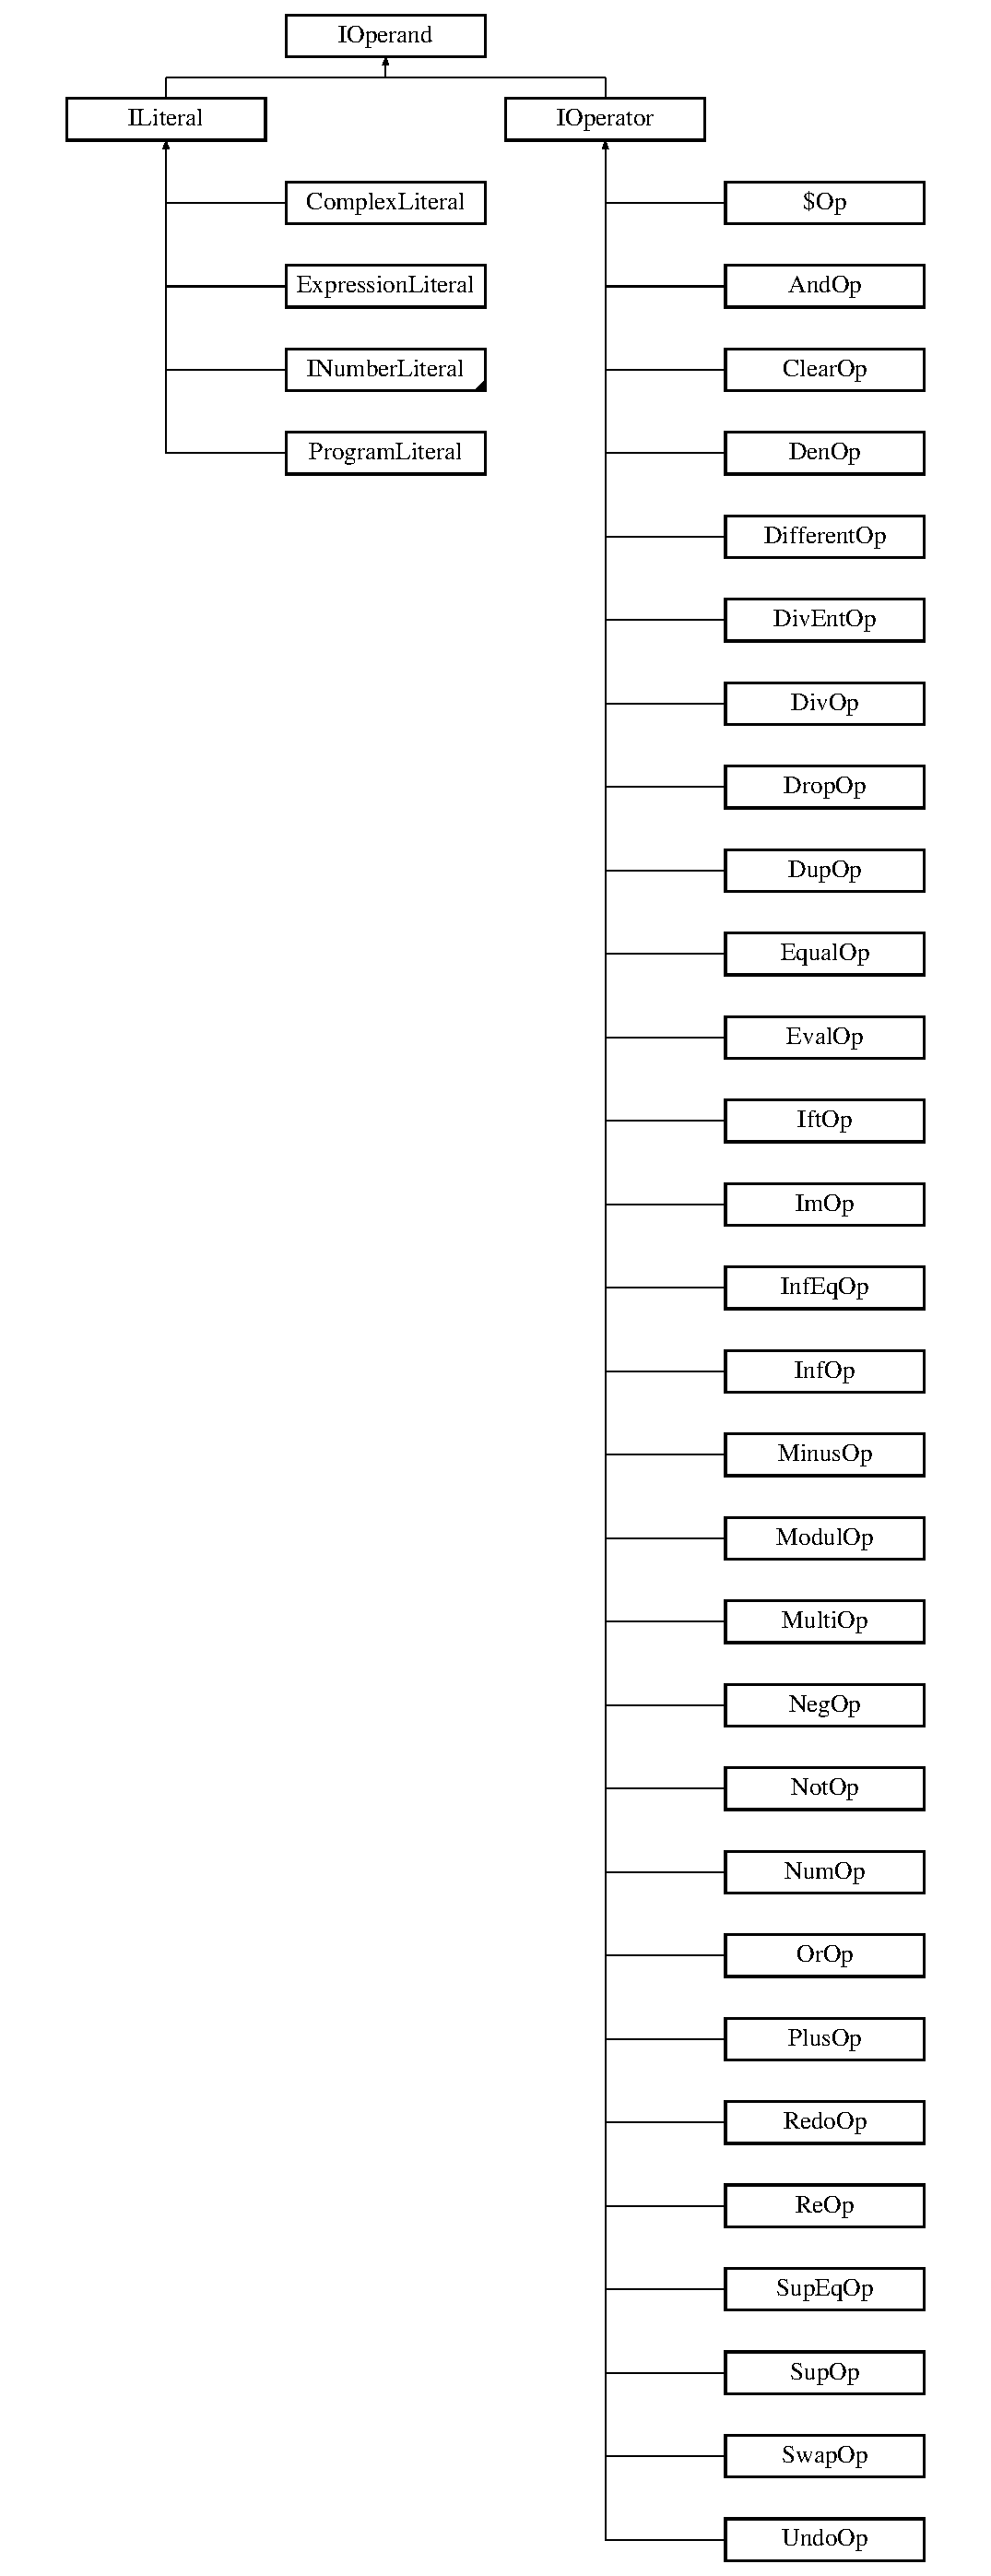
\includegraphics[height=12.000000cm]{class_i_operand}
\end{center}
\end{figure}
\subsection*{Public Member Functions}
\begin{DoxyCompactItemize}
\item 
virtual std\+::string {\bfseries to\+String} () const  =0\hypertarget{class_i_operand_a45b9e5afa570d53821d181efe4d5f333}{}\label{class_i_operand_a45b9e5afa570d53821d181efe4d5f333}

\end{DoxyCompactItemize}


The documentation for this class was generated from the following file\+:\begin{DoxyCompactItemize}
\item 
D\+:/\+Cours/\+U\+T\+C/\+P16/\+L\+O21/\+U\+T\+Computer/\+U\+T\+Computer/Literal.\+h\end{DoxyCompactItemize}

\hypertarget{class_i_operator}{}\section{I\+Operator Class Reference}
\label{class_i_operator}\index{I\+Operator@{I\+Operator}}


Classe abstraite dont chaque operateur heritera.  




{\ttfamily \#include $<$Operator.\+h$>$}

Inheritance diagram for I\+Operator\+:\begin{figure}[H]
\begin{center}
\leavevmode
\includegraphics[height=12.000000cm]{class_i_operator}
\end{center}
\end{figure}
\subsection*{Public Member Functions}
\begin{DoxyCompactItemize}
\item 
\hyperlink{class_i_operator_a7f4ccd20d66e911bcbbabcaf3fe2feec}{I\+Operator} (std\+::string s, unsigned int a)
\begin{DoxyCompactList}\small\item\em Constructeur d\textquotesingle{}un operateur. \end{DoxyCompactList}\item 
std\+::string \hyperlink{class_i_operator_a919ce3837a343f2fed1bca27e3f180e1}{to\+String} () const 
\begin{DoxyCompactList}\small\item\em Getter du symbole. \end{DoxyCompactList}\item 
virtual void \hyperlink{class_i_operator_ab93ebb15195290da26e2f3e626f6f25e}{operator()} (\hyperlink{class_stack}{Stack} $\ast$s)=0
\begin{DoxyCompactList}\small\item\em Methode virtuel redefini par chaque operator pour definir la fonction de l\textquotesingle{}operateur. \end{DoxyCompactList}\item 
unsigned int \hyperlink{class_i_operator_a2dcc556787602da06860294ad263c7a9}{get\+Arity} () const 
\begin{DoxyCompactList}\small\item\em Getter de arity. \end{DoxyCompactList}\end{DoxyCompactItemize}
\subsection*{Private Attributes}
\begin{DoxyCompactItemize}
\item 
std\+::string \hyperlink{class_i_operator_a8864ad399243cadd79da18130ca766d9}{symbol}\hypertarget{class_i_operator_a8864ad399243cadd79da18130ca766d9}{}\label{class_i_operator_a8864ad399243cadd79da18130ca766d9}

\begin{DoxyCompactList}\small\item\em Symbole utilise par l\textquotesingle{}utilisateur pour designer l\textquotesingle{}operateur. \end{DoxyCompactList}\item 
const unsigned int \hyperlink{class_i_operator_a0ac9d0762ea8f32d9e2e5c79327187c7}{arity}\hypertarget{class_i_operator_a0ac9d0762ea8f32d9e2e5c79327187c7}{}\label{class_i_operator_a0ac9d0762ea8f32d9e2e5c79327187c7}

\begin{DoxyCompactList}\small\item\em nombre d\textquotesingle{}element dont l\textquotesingle{}operateur a besoin (operateur unaire, binaire etc..) \end{DoxyCompactList}\end{DoxyCompactItemize}


\subsection{Detailed Description}
Classe abstraite dont chaque operateur heritera. 

Contient les methodes de base que chaque methode aura 

\subsection{Constructor \& Destructor Documentation}
\index{I\+Operator@{I\+Operator}!I\+Operator@{I\+Operator}}
\index{I\+Operator@{I\+Operator}!I\+Operator@{I\+Operator}}
\subsubsection[{\texorpdfstring{I\+Operator(std\+::string s, unsigned int a)}{IOperator(std::string s, unsigned int a)}}]{\setlength{\rightskip}{0pt plus 5cm}I\+Operator\+::\+I\+Operator (
\begin{DoxyParamCaption}
\item[{std\+::string}]{s, }
\item[{unsigned int}]{a}
\end{DoxyParamCaption}
)\hspace{0.3cm}{\ttfamily [inline]}}\hypertarget{class_i_operator_a7f4ccd20d66e911bcbbabcaf3fe2feec}{}\label{class_i_operator_a7f4ccd20d66e911bcbbabcaf3fe2feec}


Constructeur d\textquotesingle{}un operateur. 

Construit a partir du nom et de l\textquotesingle{}arite de l\textquotesingle{}operateur


\begin{DoxyParams}{Parameters}
{\em s} & \+: symbole designant l\textquotesingle{}operateur \\
\hline
{\em a} & \+: arite de l\textquotesingle{}operateur \\
\hline
\end{DoxyParams}


\subsection{Member Function Documentation}
\index{I\+Operator@{I\+Operator}!get\+Arity@{get\+Arity}}
\index{get\+Arity@{get\+Arity}!I\+Operator@{I\+Operator}}
\subsubsection[{\texorpdfstring{get\+Arity() const }{getArity() const }}]{\setlength{\rightskip}{0pt plus 5cm}unsigned int I\+Operator\+::get\+Arity (
\begin{DoxyParamCaption}
{}
\end{DoxyParamCaption}
) const\hspace{0.3cm}{\ttfamily [inline]}}\hypertarget{class_i_operator_a2dcc556787602da06860294ad263c7a9}{}\label{class_i_operator_a2dcc556787602da06860294ad263c7a9}


Getter de arity. 

Renvoie l\textquotesingle{}arite correspondant a l\textquotesingle{}operateur

\begin{DoxyReturn}{Returns}
std\+::string \+: arite de l\textquotesingle{}operateur 
\end{DoxyReturn}
\index{I\+Operator@{I\+Operator}!operator()@{operator()}}
\index{operator()@{operator()}!I\+Operator@{I\+Operator}}
\subsubsection[{\texorpdfstring{operator()(\+Stack $\ast$s)=0}{operator()(Stack *s)=0}}]{\setlength{\rightskip}{0pt plus 5cm}virtual void I\+Operator\+::operator() (
\begin{DoxyParamCaption}
\item[{{\bf Stack} $\ast$}]{s}
\end{DoxyParamCaption}
)\hspace{0.3cm}{\ttfamily [pure virtual]}}\hypertarget{class_i_operator_ab93ebb15195290da26e2f3e626f6f25e}{}\label{class_i_operator_ab93ebb15195290da26e2f3e626f6f25e}


Methode virtuel redefini par chaque operator pour definir la fonction de l\textquotesingle{}operateur. 

Methode principale de l\textquotesingle{}operateur \+: execute une action definie pour chaque operateur


\begin{DoxyParams}{Parameters}
{\em s} & \+: Reference sur la stack pour executer l\textquotesingle{}operateur \\
\hline
\end{DoxyParams}


Implemented in \hyperlink{class_ift_op_a189c8723b0a9ce9aee03689f6c820703}{Ift\+Op}, \hyperlink{class_eval_op_adae55ad1761c000894b6d2fc3bd7c5e4}{Eval\+Op}, \hyperlink{class_redo_op_ab90ebd24ef99001d18141c57e22a37dc}{Redo\+Op}, \hyperlink{class_undo_op_a7996f153f592410bd37aafd2e53e6527}{Undo\+Op}, \hyperlink{class_not_op_a1401d1efdc31dceb82386554ce1017d5}{Not\+Op}, \hyperlink{class_or_op_a268ddceeb945b8d8e0de436a8833efdb}{Or\+Op}, \hyperlink{class_and_op_a9d22089abf7a345221af90d050115f09}{And\+Op}, \hyperlink{class_sup_eq_op_a327405ff72000fb2e289caa82639b5a5}{Sup\+Eq\+Op}, \hyperlink{class_sup_op_a3cf5224d21e41e4e56467bafe95b0109}{Sup\+Op}, \hyperlink{class_inf_op_a9cb5e69f7534e38b8e1017ee90e65356}{Inf\+Op}, \hyperlink{class_inf_eq_op_a0ebe87e2ecf7a5f7aacefe49f7c3e8ba}{Inf\+Eq\+Op}, \hyperlink{class_different_op_a166e315a0f9b5cec5688807b6219b200}{Different\+Op}, \hyperlink{class_equal_op_a7fde70def72239e09f3127baf69c67f7}{Equal\+Op}, \hyperlink{class_clear_op_aa1175887332f472c80576559e38c105e}{Clear\+Op}, \hyperlink{class_swap_op_a70f5b133bef884968b8a9a599c4462bb}{Swap\+Op}, \hyperlink{class_drop_op_a8c357abb435073a9e4c8d421cf858cea}{Drop\+Op}, \hyperlink{class_dup_op_ad9c63f39b5fb640de5bf357726509c02}{Dup\+Op}, \hyperlink{class_im_op_a56f17f73efa21e0a5d5e082b9434296a}{Im\+Op}, \hyperlink{class_re_op_a8be9dd9930c412c7a5c3036f53423f58}{Re\+Op}, \hyperlink{class_0B_op_aee5cf8ea506c3bd12523631be240095f}{\$\+Op}, \hyperlink{class_den_op_ad7e8da512b932648c24ef95b1a534bfd}{Den\+Op}, \hyperlink{class_num_op_a353bb9b777b6201ac87c4adb41fafad0}{Num\+Op}, \hyperlink{class_neg_op_ab2be3ca4f65d893380cff95dc8e20ddb}{Neg\+Op}, \hyperlink{class_modul_op_a8dabd8f9b453c102669a009bd14f04bb}{Modul\+Op}, \hyperlink{class_div_ent_op_a18d5ddd0cfd8e1fdee438261bb3b6df4}{Div\+Ent\+Op}, \hyperlink{class_div_op_a4d68b93f7a73f40653de28e47d2d1ed2}{Div\+Op}, \hyperlink{class_multi_op_a60c1b3d35f27f08089a2ca8be8a6a7f2}{Multi\+Op}, \hyperlink{class_minus_op_a2228760c3081116bc08d59773936010a}{Minus\+Op}, and \hyperlink{class_plus_op_aff440c62f5758c5da5a08255c9518012}{Plus\+Op}.

\index{I\+Operator@{I\+Operator}!to\+String@{to\+String}}
\index{to\+String@{to\+String}!I\+Operator@{I\+Operator}}
\subsubsection[{\texorpdfstring{to\+String() const }{toString() const }}]{\setlength{\rightskip}{0pt plus 5cm}std\+::string I\+Operator\+::to\+String (
\begin{DoxyParamCaption}
{}
\end{DoxyParamCaption}
) const\hspace{0.3cm}{\ttfamily [inline]}, {\ttfamily [virtual]}}\hypertarget{class_i_operator_a919ce3837a343f2fed1bca27e3f180e1}{}\label{class_i_operator_a919ce3837a343f2fed1bca27e3f180e1}


Getter du symbole. 

Renvoie le symbole correspondant a l\textquotesingle{}operateur

\begin{DoxyReturn}{Returns}
std\+::string \+: symbole de l\textquotesingle{}operateur 
\end{DoxyReturn}


Implements \hyperlink{class_i_operand}{I\+Operand}.



The documentation for this class was generated from the following file\+:\begin{DoxyCompactItemize}
\item 
D\+:/\+Cours/\+U\+T\+C/\+P16/\+L\+O21/\+U\+T\+Computer/\+U\+T\+Computer/\hyperlink{_operator_8h}{Operator.\+h}\end{DoxyCompactItemize}

\hypertarget{class_literal_factory}{}\section{Literal\+Factory Class Reference}
\label{class_literal_factory}\index{Literal\+Factory@{Literal\+Factory}}
\subsection*{Public Member Functions}
\begin{DoxyCompactItemize}
\item 
{\bfseries Literal\+Factory} (const \hyperlink{class_literal_factory}{Literal\+Factory} \&)=delete\hypertarget{class_literal_factory_a5077bb918d1bb4602e187fcdc0233594}{}\label{class_literal_factory_a5077bb918d1bb4602e187fcdc0233594}

\item 
void {\bfseries operator=} (const \hyperlink{class_literal_factory}{Literal\+Factory} \&)=delete\hypertarget{class_literal_factory_a50b8f3d96ec5f50506da79392c57647a}{}\label{class_literal_factory_a50b8f3d96ec5f50506da79392c57647a}

\item 
\hyperlink{class_i_literal}{I\+Literal} $\ast$ {\bfseries make\+Literal} (int n) const \hypertarget{class_literal_factory_a2c247f6ffc8fb323390317eea0ff2f37}{}\label{class_literal_factory_a2c247f6ffc8fb323390317eea0ff2f37}

\item 
\hyperlink{class_i_literal}{I\+Literal} $\ast$ {\bfseries make\+Literal} (double n) const \hypertarget{class_literal_factory_abfeac7e7cee838e62e9f1f3062b46521}{}\label{class_literal_factory_abfeac7e7cee838e62e9f1f3062b46521}

\item 
\hyperlink{class_i_literal}{I\+Literal} $\ast$ {\bfseries make\+Literal} (std\+::pair$<$ int, int $>$ n) const \hypertarget{class_literal_factory_a08c37b9b29232ea4ca50a5e74420ece5}{}\label{class_literal_factory_a08c37b9b29232ea4ca50a5e74420ece5}

\item 
\hyperlink{class_i_literal}{I\+Literal} $\ast$ {\bfseries make\+Literal} (\hyperlink{class_i_number_literal}{I\+Number\+Literal} $\ast$re, \hyperlink{class_i_number_literal}{I\+Number\+Literal} $\ast$im) const \hypertarget{class_literal_factory_a9f4a084c4fbe6b7b39506e3483d953fd}{}\label{class_literal_factory_a9f4a084c4fbe6b7b39506e3483d953fd}

\item 
\hyperlink{class_i_literal}{I\+Literal} $\ast$ {\bfseries make\+Literal} (std\+::string str) const \hypertarget{class_literal_factory_a81d6cea1140f102801eb652a15e9196c}{}\label{class_literal_factory_a81d6cea1140f102801eb652a15e9196c}

\end{DoxyCompactItemize}
\subsection*{Static Public Member Functions}
\begin{DoxyCompactItemize}
\item 
static const \hyperlink{class_literal_factory}{Literal\+Factory} \& {\bfseries get\+Instance} ()\hypertarget{class_literal_factory_aec9768d18ca1f1b46c9718825be9f364}{}\label{class_literal_factory_aec9768d18ca1f1b46c9718825be9f364}

\end{DoxyCompactItemize}
\subsection*{Private Member Functions}
\begin{DoxyCompactItemize}
\item 
\hyperlink{class_i_number_literal}{I\+Number\+Literal} $\ast$ {\bfseries make\+Number\+Literal} (std\+::string str) const \hypertarget{class_literal_factory_abdfc288d8f0d4c869e0fbb21f08223e4}{}\label{class_literal_factory_abdfc288d8f0d4c869e0fbb21f08223e4}

\end{DoxyCompactItemize}


The documentation for this class was generated from the following files\+:\begin{DoxyCompactItemize}
\item 
D\+:/\+Cours/\+U\+T\+C/\+P16/\+L\+O21/\+U\+T\+Computer/\+U\+T\+Computer/Literal\+Factory.\+h\item 
D\+:/\+Cours/\+U\+T\+C/\+P16/\+L\+O21/\+U\+T\+Computer/\+U\+T\+Computer/Literal\+Factory.\+cpp\end{DoxyCompactItemize}

\hypertarget{class_minus_op}{}\section{Minus\+Op Class Reference}
\label{class_minus_op}\index{Minus\+Op@{Minus\+Op}}


Execute le deuxi�me element -\/ le premier.  




{\ttfamily \#include $<$Operator.\+h$>$}

Inheritance diagram for Minus\+Op\+:\begin{figure}[H]
\begin{center}
\leavevmode
\includegraphics[height=3.000000cm]{class_minus_op}
\end{center}
\end{figure}
\subsection*{Public Member Functions}
\begin{DoxyCompactItemize}
\item 
\hyperlink{class_minus_op_aa895504ffa16e1e9cb52678ec04636ea}{Minus\+Op} ()
\begin{DoxyCompactList}\small\item\em Constructeur de l\textquotesingle{}operateur. \end{DoxyCompactList}\item 
void \hyperlink{class_minus_op_a2228760c3081116bc08d59773936010a}{operator()} (\hyperlink{class_stack}{Stack} $\ast$s)
\begin{DoxyCompactList}\small\item\em Methode virtuel redefini par chaque operator pour definir la fonction de l\textquotesingle{}operateur. \end{DoxyCompactList}\end{DoxyCompactItemize}


\subsection{Detailed Description}
Execute le deuxi�me element -\/ le premier. 

Permet de soustraite les deux premiers element de la pile 

\subsection{Constructor \& Destructor Documentation}
\index{Minus\+Op@{Minus\+Op}!Minus\+Op@{Minus\+Op}}
\index{Minus\+Op@{Minus\+Op}!Minus\+Op@{Minus\+Op}}
\subsubsection[{\texorpdfstring{Minus\+Op()}{MinusOp()}}]{\setlength{\rightskip}{0pt plus 5cm}Minus\+Op\+::\+Minus\+Op (
\begin{DoxyParamCaption}
{}
\end{DoxyParamCaption}
)\hspace{0.3cm}{\ttfamily [inline]}}\hypertarget{class_minus_op_aa895504ffa16e1e9cb52678ec04636ea}{}\label{class_minus_op_aa895504ffa16e1e9cb52678ec04636ea}


Constructeur de l\textquotesingle{}operateur. 

Construit l\textquotesingle{}operateur avec le symbole -\/ et arit� 2 

\subsection{Member Function Documentation}
\index{Minus\+Op@{Minus\+Op}!operator()@{operator()}}
\index{operator()@{operator()}!Minus\+Op@{Minus\+Op}}
\subsubsection[{\texorpdfstring{operator()(\+Stack $\ast$s)}{operator()(Stack *s)}}]{\setlength{\rightskip}{0pt plus 5cm}void Minus\+Op\+::operator() (
\begin{DoxyParamCaption}
\item[{{\bf Stack} $\ast$}]{s}
\end{DoxyParamCaption}
)\hspace{0.3cm}{\ttfamily [virtual]}}\hypertarget{class_minus_op_a2228760c3081116bc08d59773936010a}{}\label{class_minus_op_a2228760c3081116bc08d59773936010a}


Methode virtuel redefini par chaque operator pour definir la fonction de l\textquotesingle{}operateur. 

Methode principale de l\textquotesingle{}operateur \+: execute une action definie pour chaque operateur


\begin{DoxyParams}{Parameters}
{\em s} & \+: Reference sur la stack pour executer l\textquotesingle{}operateur \\
\hline
\end{DoxyParams}


Implements \hyperlink{class_i_operator_ab93ebb15195290da26e2f3e626f6f25e}{I\+Operator}.



The documentation for this class was generated from the following files\+:\begin{DoxyCompactItemize}
\item 
D\+:/\+Cours/\+U\+T\+C/\+P16/\+L\+O21/\+U\+T\+Computer/\+U\+T\+Computer/\hyperlink{_operator_8h}{Operator.\+h}\item 
D\+:/\+Cours/\+U\+T\+C/\+P16/\+L\+O21/\+U\+T\+Computer/\+U\+T\+Computer/Operator.\+cpp\end{DoxyCompactItemize}

\hypertarget{class_modul_op}{}\section{Modul\+Op Class Reference}
\label{class_modul_op}\index{Modul\+Op@{Modul\+Op}}


Modulo du premier element par le deuxieme.  




{\ttfamily \#include $<$Operator.\+h$>$}

Inheritance diagram for Modul\+Op\+:\begin{figure}[H]
\begin{center}
\leavevmode
\includegraphics[height=3.000000cm]{class_modul_op}
\end{center}
\end{figure}
\subsection*{Public Member Functions}
\begin{DoxyCompactItemize}
\item 
\hyperlink{class_modul_op_aec69fad637ebf3c144862cb90b42a2cb}{Modul\+Op} ()
\begin{DoxyCompactList}\small\item\em Constructeur de l\textquotesingle{}operateur. \end{DoxyCompactList}\item 
void \hyperlink{class_modul_op_a8dabd8f9b453c102669a009bd14f04bb}{operator()} (\hyperlink{class_stack}{Stack} $\ast$s)
\begin{DoxyCompactList}\small\item\em Methode virtuel redefini par chaque operator pour definir la fonction de l\textquotesingle{}operateur. \end{DoxyCompactList}\end{DoxyCompactItemize}


\subsection{Detailed Description}
Modulo du premier element par le deuxieme. 

Permet de renvoyer le reste du modulo d\textquotesingle{}un nombre par un autre 

\subsection{Constructor \& Destructor Documentation}
\index{Modul\+Op@{Modul\+Op}!Modul\+Op@{Modul\+Op}}
\index{Modul\+Op@{Modul\+Op}!Modul\+Op@{Modul\+Op}}
\subsubsection[{\texorpdfstring{Modul\+Op()}{ModulOp()}}]{\setlength{\rightskip}{0pt plus 5cm}Modul\+Op\+::\+Modul\+Op (
\begin{DoxyParamCaption}
{}
\end{DoxyParamCaption}
)\hspace{0.3cm}{\ttfamily [inline]}}\hypertarget{class_modul_op_aec69fad637ebf3c144862cb90b42a2cb}{}\label{class_modul_op_aec69fad637ebf3c144862cb90b42a2cb}


Constructeur de l\textquotesingle{}operateur. 

Construit l\textquotesingle{}operateur avec le symbole M\+OD et arit� 2 

\subsection{Member Function Documentation}
\index{Modul\+Op@{Modul\+Op}!operator()@{operator()}}
\index{operator()@{operator()}!Modul\+Op@{Modul\+Op}}
\subsubsection[{\texorpdfstring{operator()(\+Stack $\ast$s)}{operator()(Stack *s)}}]{\setlength{\rightskip}{0pt plus 5cm}void Modul\+Op\+::operator() (
\begin{DoxyParamCaption}
\item[{{\bf Stack} $\ast$}]{s}
\end{DoxyParamCaption}
)\hspace{0.3cm}{\ttfamily [virtual]}}\hypertarget{class_modul_op_a8dabd8f9b453c102669a009bd14f04bb}{}\label{class_modul_op_a8dabd8f9b453c102669a009bd14f04bb}


Methode virtuel redefini par chaque operator pour definir la fonction de l\textquotesingle{}operateur. 

Methode principale de l\textquotesingle{}operateur \+: execute une action definie pour chaque operateur


\begin{DoxyParams}{Parameters}
{\em s} & \+: Reference sur la stack pour executer l\textquotesingle{}operateur \\
\hline
\end{DoxyParams}


Implements \hyperlink{class_i_operator_ab93ebb15195290da26e2f3e626f6f25e}{I\+Operator}.



The documentation for this class was generated from the following files\+:\begin{DoxyCompactItemize}
\item 
D\+:/\+Cours/\+U\+T\+C/\+P16/\+L\+O21/\+U\+T\+Computer/\+U\+T\+Computer/\hyperlink{_operator_8h}{Operator.\+h}\item 
D\+:/\+Cours/\+U\+T\+C/\+P16/\+L\+O21/\+U\+T\+Computer/\+U\+T\+Computer/Operator.\+cpp\end{DoxyCompactItemize}

\hypertarget{class_multi_op}{}\section{Multi\+Op Class Reference}
\label{class_multi_op}\index{Multi\+Op@{Multi\+Op}}


Execute \textquotesingle{}$\ast$\textquotesingle{} sur les deux premiers element de la pile.  




{\ttfamily \#include $<$Operator.\+h$>$}

Inheritance diagram for Multi\+Op\+:\begin{figure}[H]
\begin{center}
\leavevmode
\includegraphics[height=3.000000cm]{class_multi_op}
\end{center}
\end{figure}
\subsection*{Public Member Functions}
\begin{DoxyCompactItemize}
\item 
\hyperlink{class_multi_op_a1023543d1d548e4485e5e8edc54118dd}{Multi\+Op} ()
\begin{DoxyCompactList}\small\item\em Constructeur de l\textquotesingle{}operateur. \end{DoxyCompactList}\item 
void \hyperlink{class_multi_op_a60c1b3d35f27f08089a2ca8be8a6a7f2}{operator()} (\hyperlink{class_stack}{Stack} $\ast$s)
\begin{DoxyCompactList}\small\item\em Methode virtuel redefini par chaque operator pour definir la fonction de l\textquotesingle{}operateur. \end{DoxyCompactList}\end{DoxyCompactItemize}


\subsection{Detailed Description}
Execute \textquotesingle{}$\ast$\textquotesingle{} sur les deux premiers element de la pile. 

Permet de multiplier les deux premiers element de la pile 

\subsection{Constructor \& Destructor Documentation}
\index{Multi\+Op@{Multi\+Op}!Multi\+Op@{Multi\+Op}}
\index{Multi\+Op@{Multi\+Op}!Multi\+Op@{Multi\+Op}}
\subsubsection[{\texorpdfstring{Multi\+Op()}{MultiOp()}}]{\setlength{\rightskip}{0pt plus 5cm}Multi\+Op\+::\+Multi\+Op (
\begin{DoxyParamCaption}
{}
\end{DoxyParamCaption}
)\hspace{0.3cm}{\ttfamily [inline]}}\hypertarget{class_multi_op_a1023543d1d548e4485e5e8edc54118dd}{}\label{class_multi_op_a1023543d1d548e4485e5e8edc54118dd}


Constructeur de l\textquotesingle{}operateur. 

Construit l\textquotesingle{}operateur avec le symbole $\ast$ et arit� 2 

\subsection{Member Function Documentation}
\index{Multi\+Op@{Multi\+Op}!operator()@{operator()}}
\index{operator()@{operator()}!Multi\+Op@{Multi\+Op}}
\subsubsection[{\texorpdfstring{operator()(\+Stack $\ast$s)}{operator()(Stack *s)}}]{\setlength{\rightskip}{0pt plus 5cm}void Multi\+Op\+::operator() (
\begin{DoxyParamCaption}
\item[{{\bf Stack} $\ast$}]{s}
\end{DoxyParamCaption}
)\hspace{0.3cm}{\ttfamily [virtual]}}\hypertarget{class_multi_op_a60c1b3d35f27f08089a2ca8be8a6a7f2}{}\label{class_multi_op_a60c1b3d35f27f08089a2ca8be8a6a7f2}


Methode virtuel redefini par chaque operator pour definir la fonction de l\textquotesingle{}operateur. 

Methode principale de l\textquotesingle{}operateur \+: execute une action definie pour chaque operateur


\begin{DoxyParams}{Parameters}
{\em s} & \+: Reference sur la stack pour executer l\textquotesingle{}operateur \\
\hline
\end{DoxyParams}


Implements \hyperlink{class_i_operator_ab93ebb15195290da26e2f3e626f6f25e}{I\+Operator}.



The documentation for this class was generated from the following files\+:\begin{DoxyCompactItemize}
\item 
D\+:/\+Cours/\+U\+T\+C/\+P16/\+L\+O21/\+U\+T\+Computer/\+U\+T\+Computer/\hyperlink{_operator_8h}{Operator.\+h}\item 
D\+:/\+Cours/\+U\+T\+C/\+P16/\+L\+O21/\+U\+T\+Computer/\+U\+T\+Computer/Operator.\+cpp\end{DoxyCompactItemize}

\hypertarget{class_neg_op}{}\section{Neg\+Op Class Reference}
\label{class_neg_op}\index{Neg\+Op@{Neg\+Op}}


Permet de changer le signe d\textquotesingle{}une valeur.  




{\ttfamily \#include $<$Operator.\+h$>$}

Inheritance diagram for Neg\+Op\+:\begin{figure}[H]
\begin{center}
\leavevmode
\includegraphics[height=3.000000cm]{class_neg_op}
\end{center}
\end{figure}
\subsection*{Public Member Functions}
\begin{DoxyCompactItemize}
\item 
\hyperlink{class_neg_op_a6ccfa67bc9837f48d3852a7ab2c13db5}{Neg\+Op} ()
\begin{DoxyCompactList}\small\item\em Constructeur de l\textquotesingle{}operateur. \end{DoxyCompactList}\item 
void \hyperlink{class_neg_op_ab2be3ca4f65d893380cff95dc8e20ddb}{operator()} (\hyperlink{class_stack}{Stack} $\ast$s)
\begin{DoxyCompactList}\small\item\em Methode virtuel redefini par chaque operator pour definir la fonction de l\textquotesingle{}operateur. \end{DoxyCompactList}\end{DoxyCompactItemize}


\subsection{Detailed Description}
Permet de changer le signe d\textquotesingle{}une valeur. 

Met dans la pile la premiere valeur de celle ci en changeant son signe 

\subsection{Constructor \& Destructor Documentation}
\index{Neg\+Op@{Neg\+Op}!Neg\+Op@{Neg\+Op}}
\index{Neg\+Op@{Neg\+Op}!Neg\+Op@{Neg\+Op}}
\subsubsection[{\texorpdfstring{Neg\+Op()}{NegOp()}}]{\setlength{\rightskip}{0pt plus 5cm}Neg\+Op\+::\+Neg\+Op (
\begin{DoxyParamCaption}
{}
\end{DoxyParamCaption}
)\hspace{0.3cm}{\ttfamily [inline]}}\hypertarget{class_neg_op_a6ccfa67bc9837f48d3852a7ab2c13db5}{}\label{class_neg_op_a6ccfa67bc9837f48d3852a7ab2c13db5}


Constructeur de l\textquotesingle{}operateur. 

Construit l\textquotesingle{}operateur avec le symbole N\+EG et arit� 1 

\subsection{Member Function Documentation}
\index{Neg\+Op@{Neg\+Op}!operator()@{operator()}}
\index{operator()@{operator()}!Neg\+Op@{Neg\+Op}}
\subsubsection[{\texorpdfstring{operator()(\+Stack $\ast$s)}{operator()(Stack *s)}}]{\setlength{\rightskip}{0pt plus 5cm}void Neg\+Op\+::operator() (
\begin{DoxyParamCaption}
\item[{{\bf Stack} $\ast$}]{s}
\end{DoxyParamCaption}
)\hspace{0.3cm}{\ttfamily [virtual]}}\hypertarget{class_neg_op_ab2be3ca4f65d893380cff95dc8e20ddb}{}\label{class_neg_op_ab2be3ca4f65d893380cff95dc8e20ddb}


Methode virtuel redefini par chaque operator pour definir la fonction de l\textquotesingle{}operateur. 

Methode principale de l\textquotesingle{}operateur \+: execute une action definie pour chaque operateur


\begin{DoxyParams}{Parameters}
{\em s} & \+: Reference sur la stack pour executer l\textquotesingle{}operateur \\
\hline
\end{DoxyParams}


Implements \hyperlink{class_i_operator_ab93ebb15195290da26e2f3e626f6f25e}{I\+Operator}.



The documentation for this class was generated from the following files\+:\begin{DoxyCompactItemize}
\item 
D\+:/\+Cours/\+U\+T\+C/\+P16/\+L\+O21/\+U\+T\+Computer/\+U\+T\+Computer/\hyperlink{_operator_8h}{Operator.\+h}\item 
D\+:/\+Cours/\+U\+T\+C/\+P16/\+L\+O21/\+U\+T\+Computer/\+U\+T\+Computer/Operator.\+cpp\end{DoxyCompactItemize}

\input{class_not_op}
\hypertarget{class_num_op}{}\section{Num\+Op Class Reference}
\label{class_num_op}\index{Num\+Op@{Num\+Op}}
Inheritance diagram for Num\+Op\+:\begin{figure}[H]
\begin{center}
\leavevmode
\includegraphics[height=3.000000cm]{class_num_op}
\end{center}
\end{figure}
\subsection*{Public Member Functions}
\begin{DoxyCompactItemize}
\item 
void \hyperlink{class_num_op_a353bb9b777b6201ac87c4adb41fafad0}{operator()} (\hyperlink{class_stack}{Stack} $\ast$s)
\begin{DoxyCompactList}\small\item\em Methode virtuel redefini par chaque operator pour definir la fonction de l\textquotesingle{}operateur. \end{DoxyCompactList}\end{DoxyCompactItemize}


\subsection{Member Function Documentation}
\index{Num\+Op@{Num\+Op}!operator()@{operator()}}
\index{operator()@{operator()}!Num\+Op@{Num\+Op}}
\subsubsection[{\texorpdfstring{operator()(\+Stack $\ast$s)}{operator()(Stack *s)}}]{\setlength{\rightskip}{0pt plus 5cm}void Num\+Op\+::operator() (
\begin{DoxyParamCaption}
\item[{{\bf Stack} $\ast$}]{s}
\end{DoxyParamCaption}
)\hspace{0.3cm}{\ttfamily [virtual]}}\hypertarget{class_num_op_a353bb9b777b6201ac87c4adb41fafad0}{}\label{class_num_op_a353bb9b777b6201ac87c4adb41fafad0}


Methode virtuel redefini par chaque operator pour definir la fonction de l\textquotesingle{}operateur. 

Methode principale de l\textquotesingle{}operateur \+: execute une action definie pour chaque operateur


\begin{DoxyParams}{Parameters}
{\em s} & \+: Reference sur la stack pour executer l\textquotesingle{}operateur \\
\hline
\end{DoxyParams}


Implements \hyperlink{class_i_operator_ab93ebb15195290da26e2f3e626f6f25e}{I\+Operator}.



The documentation for this class was generated from the following files\+:\begin{DoxyCompactItemize}
\item 
D\+:/\+Cours/\+U\+T\+C/\+P16/\+L\+O21/\+U\+T\+Computer/\+U\+T\+Computer/\hyperlink{_operator_8h}{Operator.\+h}\item 
D\+:/\+Cours/\+U\+T\+C/\+P16/\+L\+O21/\+U\+T\+Computer/\+U\+T\+Computer/Operator.\+cpp\end{DoxyCompactItemize}

\hypertarget{class_operator_exception}{}\section{Operator\+Exception Class Reference}
\label{class_operator_exception}\index{Operator\+Exception@{Operator\+Exception}}
\subsection*{Public Member Functions}
\begin{DoxyCompactItemize}
\item 
{\bfseries Operator\+Exception} (const std\+::string \&str)\hypertarget{class_operator_exception_a0a3e109c75dc9c9e8db314399585c5d1}{}\label{class_operator_exception_a0a3e109c75dc9c9e8db314399585c5d1}

\item 
std\+::string {\bfseries get\+Info} () const \hypertarget{class_operator_exception_ad9658cb08568b91c6e5ac86ce51c59b7}{}\label{class_operator_exception_ad9658cb08568b91c6e5ac86ce51c59b7}

\end{DoxyCompactItemize}
\subsection*{Private Attributes}
\begin{DoxyCompactItemize}
\item 
std\+::string {\bfseries info}\hypertarget{class_operator_exception_aebc5f900bf87e1c83c3e2980aae22790}{}\label{class_operator_exception_aebc5f900bf87e1c83c3e2980aae22790}

\end{DoxyCompactItemize}


The documentation for this class was generated from the following file\+:\begin{DoxyCompactItemize}
\item 
D\+:/\+Cours/\+U\+T\+C/\+P16/\+L\+O21/\+U\+T\+Computer/\+U\+T\+Computer/Operator\+Exception.\+h\end{DoxyCompactItemize}

\input{class_or_op}
\hypertarget{class_plus_op}{}\section{Plus\+Op Class Reference}
\label{class_plus_op}\index{Plus\+Op@{Plus\+Op}}


Execute \textquotesingle{}+\textquotesingle{} sur les deux premiers element de la pile.  




{\ttfamily \#include $<$Operator.\+h$>$}

Inheritance diagram for Plus\+Op\+:\begin{figure}[H]
\begin{center}
\leavevmode
\includegraphics[height=3.000000cm]{class_plus_op}
\end{center}
\end{figure}
\subsection*{Public Member Functions}
\begin{DoxyCompactItemize}
\item 
\hyperlink{class_plus_op_a5a8d41dcc72cfcb807ccbc9a55734b3f}{Plus\+Op} ()
\begin{DoxyCompactList}\small\item\em Constructeur de l\textquotesingle{}operateur. \end{DoxyCompactList}\item 
void \hyperlink{class_plus_op_aff440c62f5758c5da5a08255c9518012}{operator()} (\hyperlink{class_stack}{Stack} $\ast$s)
\begin{DoxyCompactList}\small\item\em Methode virtuel redefini par chaque operator pour definir la fonction de l\textquotesingle{}operateur. \end{DoxyCompactList}\end{DoxyCompactItemize}


\subsection{Detailed Description}
Execute \textquotesingle{}+\textquotesingle{} sur les deux premiers element de la pile. 

Permet d\textquotesingle{}additionner les deux premiers element de la pile 

\subsection{Constructor \& Destructor Documentation}
\index{Plus\+Op@{Plus\+Op}!Plus\+Op@{Plus\+Op}}
\index{Plus\+Op@{Plus\+Op}!Plus\+Op@{Plus\+Op}}
\subsubsection[{\texorpdfstring{Plus\+Op()}{PlusOp()}}]{\setlength{\rightskip}{0pt plus 5cm}Plus\+Op\+::\+Plus\+Op (
\begin{DoxyParamCaption}
{}
\end{DoxyParamCaption}
)\hspace{0.3cm}{\ttfamily [inline]}}\hypertarget{class_plus_op_a5a8d41dcc72cfcb807ccbc9a55734b3f}{}\label{class_plus_op_a5a8d41dcc72cfcb807ccbc9a55734b3f}


Constructeur de l\textquotesingle{}operateur. 

Construit l\textquotesingle{}operateur avec le symbole + et arit� 2 

\subsection{Member Function Documentation}
\index{Plus\+Op@{Plus\+Op}!operator()@{operator()}}
\index{operator()@{operator()}!Plus\+Op@{Plus\+Op}}
\subsubsection[{\texorpdfstring{operator()(\+Stack $\ast$s)}{operator()(Stack *s)}}]{\setlength{\rightskip}{0pt plus 5cm}void Plus\+Op\+::operator() (
\begin{DoxyParamCaption}
\item[{{\bf Stack} $\ast$}]{s}
\end{DoxyParamCaption}
)\hspace{0.3cm}{\ttfamily [virtual]}}\hypertarget{class_plus_op_aff440c62f5758c5da5a08255c9518012}{}\label{class_plus_op_aff440c62f5758c5da5a08255c9518012}


Methode virtuel redefini par chaque operator pour definir la fonction de l\textquotesingle{}operateur. 

Methode principale de l\textquotesingle{}operateur \+: execute une action definie pour chaque operateur


\begin{DoxyParams}{Parameters}
{\em s} & \+: Reference sur la stack pour executer l\textquotesingle{}operateur \\
\hline
\end{DoxyParams}


Implements \hyperlink{class_i_operator_ab93ebb15195290da26e2f3e626f6f25e}{I\+Operator}.



The documentation for this class was generated from the following files\+:\begin{DoxyCompactItemize}
\item 
D\+:/\+Cours/\+U\+T\+C/\+P16/\+L\+O21/\+U\+T\+Computer/\+U\+T\+Computer/\hyperlink{_operator_8h}{Operator.\+h}\item 
D\+:/\+Cours/\+U\+T\+C/\+P16/\+L\+O21/\+U\+T\+Computer/\+U\+T\+Computer/Operator.\+cpp\end{DoxyCompactItemize}

\hypertarget{class_program_literal}{}\section{Program\+Literal Class Reference}
\label{class_program_literal}\index{Program\+Literal@{Program\+Literal}}
Inheritance diagram for Program\+Literal\+:\begin{figure}[H]
\begin{center}
\leavevmode
\includegraphics[height=3.000000cm]{class_program_literal}
\end{center}
\end{figure}
\subsection*{Public Member Functions}
\begin{DoxyCompactItemize}
\item 
{\bfseries Program\+Literal} (std\+::string p)\hypertarget{class_program_literal_a19ac6600917aa34bf41374f9b77c5400}{}\label{class_program_literal_a19ac6600917aa34bf41374f9b77c5400}

\item 
\hyperlink{class_i_literal}{I\+Literal} $\ast$ {\bfseries clone} () const \hypertarget{class_program_literal_a19b986a859b88240600e444ad8534437}{}\label{class_program_literal_a19b986a859b88240600e444ad8534437}

\item 
std\+::string {\bfseries get\+Value} () const \hypertarget{class_program_literal_ae2b1010037bbd8991c937a2eda623ad6}{}\label{class_program_literal_ae2b1010037bbd8991c937a2eda623ad6}

\item 
std\+::string {\bfseries to\+String} () const \hypertarget{class_program_literal_a8ad99a9d8755d1637e30b79ae55f7f25}{}\label{class_program_literal_a8ad99a9d8755d1637e30b79ae55f7f25}

\item 
bool {\bfseries is\+Nul} () const \hypertarget{class_program_literal_ad12118745d3b3d30d700a7fcca02d4d7}{}\label{class_program_literal_ad12118745d3b3d30d700a7fcca02d4d7}

\end{DoxyCompactItemize}
\subsection*{Private Attributes}
\begin{DoxyCompactItemize}
\item 
std\+::string {\bfseries program}\hypertarget{class_program_literal_a85093db30df36b13a6f435a5856ffa3f}{}\label{class_program_literal_a85093db30df36b13a6f435a5856ffa3f}

\end{DoxyCompactItemize}


The documentation for this class was generated from the following file\+:\begin{DoxyCompactItemize}
\item 
D\+:/\+Cours/\+U\+T\+C/\+P16/\+L\+O21/\+U\+T\+Computer/\+U\+T\+Computer/Literal.\+h\end{DoxyCompactItemize}

\hypertarget{class_q_computer}{}\section{Q\+Computer Class Reference}
\label{class_q_computer}\index{Q\+Computer@{Q\+Computer}}
Inheritance diagram for Q\+Computer\+:\begin{figure}[H]
\begin{center}
\leavevmode
\includegraphics[height=2.000000cm]{class_q_computer}
\end{center}
\end{figure}
\subsection*{Public Slots}
\begin{DoxyCompactItemize}
\item 
void {\bfseries refresh} ()\hypertarget{class_q_computer_a511996271d43631e5296f62becc2962a}{}\label{class_q_computer_a511996271d43631e5296f62becc2962a}

\item 
void {\bfseries get\+Next\+Commande} ()\hypertarget{class_q_computer_ac32346fc787c1b6fea066f26c9a24e69}{}\label{class_q_computer_ac32346fc787c1b6fea066f26c9a24e69}

\item 
void {\bfseries print\+Error} (std\+::string error)\hypertarget{class_q_computer_a8e2e06c55204647b4e25ca34aad27301}{}\label{class_q_computer_a8e2e06c55204647b4e25ca34aad27301}

\item 
void {\bfseries set\+Texte} ()\hypertarget{class_q_computer_a985f32ad67bd2fe5e3786df9b2347596}{}\label{class_q_computer_a985f32ad67bd2fe5e3786df9b2347596}

\item 
void {\bfseries desactiver\+Bip} ()\hypertarget{class_q_computer_a01da83a084b0551b5fa02db509385bb2}{}\label{class_q_computer_a01da83a084b0551b5fa02db509385bb2}

\item 
void {\bfseries choix\+Nombre\+Variable} ()\hypertarget{class_q_computer_a757164ed84f768a9dcf12b7bd9ff219b}{}\label{class_q_computer_a757164ed84f768a9dcf12b7bd9ff219b}

\item 
void {\bfseries desactiver\+Cliquable} ()\hypertarget{class_q_computer_a043ecc5f78d8a7d988468782e11881e1}{}\label{class_q_computer_a043ecc5f78d8a7d988468782e11881e1}

\item 
void {\bfseries call\+Operator} ()\hypertarget{class_q_computer_af0133edd19574e8bbfa97b62fe6deb12}{}\label{class_q_computer_af0133edd19574e8bbfa97b62fe6deb12}

\item 
void {\bfseries creation\+Var} ()\hypertarget{class_q_computer_af3e243b9d24bf70bb30f101d25048b61}{}\label{class_q_computer_af3e243b9d24bf70bb30f101d25048b61}

\item 
void {\bfseries modif\+Var} (std\+::string name=\char`\"{}\char`\"{})\hypertarget{class_q_computer_a704a6f1045c05e3df28d27e2f22f260d}{}\label{class_q_computer_a704a6f1045c05e3df28d27e2f22f260d}

\item 
void {\bfseries supprimer\+Var} ()\hypertarget{class_q_computer_a4b791644c20c3a13e9b1f99a87e06b8e}{}\label{class_q_computer_a4b791644c20c3a13e9b1f99a87e06b8e}

\item 
void {\bfseries creation\+Fct} ()\hypertarget{class_q_computer_ab39575bd54a88e802e1ee3c8e9615698}{}\label{class_q_computer_ab39575bd54a88e802e1ee3c8e9615698}

\item 
void {\bfseries modif\+Fct} (std\+::string name=\char`\"{}\char`\"{})\hypertarget{class_q_computer_a83be6904746d61a0bc140de79c11dbd9}{}\label{class_q_computer_a83be6904746d61a0bc140de79c11dbd9}

\item 
void {\bfseries supprimer\+Fct} ()\hypertarget{class_q_computer_a7c042b5ef0fb53d5339ce6bfc4f606d0}{}\label{class_q_computer_a7c042b5ef0fb53d5339ce6bfc4f606d0}

\item 
void {\bfseries set\+Variable} (Q\+String value)\hypertarget{class_q_computer_abc85a4ac72f7589708ab3478921821ff}{}\label{class_q_computer_abc85a4ac72f7589708ab3478921821ff}

\item 
void {\bfseries set\+Fct} ()\hypertarget{class_q_computer_a35059026af9cb530bafcd44516c33541}{}\label{class_q_computer_a35059026af9cb530bafcd44516c33541}

\item 
void {\bfseries save\+And\+Quit} ()\hypertarget{class_q_computer_a57ae10dd6f6eb43cd7c40776b6c81a27}{}\label{class_q_computer_a57ae10dd6f6eb43cd7c40776b6c81a27}

\item 
void {\bfseries execute\+CtrlZ} ()\hypertarget{class_q_computer_a045ff0a9634978deff477562dbdde2ba}{}\label{class_q_computer_a045ff0a9634978deff477562dbdde2ba}

\item 
void {\bfseries execute\+CtrlY} ()\hypertarget{class_q_computer_a19abf696fe84544ed0eb0798520cdcee}{}\label{class_q_computer_a19abf696fe84544ed0eb0798520cdcee}

\end{DoxyCompactItemize}
\subsection*{Public Member Functions}
\begin{DoxyCompactItemize}
\item 
{\bfseries Q\+Computer} (Q\+Widget $\ast$parent=0)\hypertarget{class_q_computer_a3a71a18fabd57942cf0d85a916d31624}{}\label{class_q_computer_a3a71a18fabd57942cf0d85a916d31624}

\item 
void {\bfseries create\+Operator\+Action} ()\hypertarget{class_q_computer_aa8efe96b7342f9e32778658fe6964565}{}\label{class_q_computer_aa8efe96b7342f9e32778658fe6964565}

\item 
void {\bfseries create\+Var\+And\+Prog\+Action} ()\hypertarget{class_q_computer_a1ffbe2fffbe11e7916f599337f51b805}{}\label{class_q_computer_a1ffbe2fffbe11e7916f599337f51b805}

\item 
void {\bfseries close\+Event} (Q\+Close\+Event $\ast$event)\hypertarget{class_q_computer_aec79b2c7edaa9637eb83d4e5f2f369c8}{}\label{class_q_computer_aec79b2c7edaa9637eb83d4e5f2f369c8}

\end{DoxyCompactItemize}
\subsection*{Private Attributes}
\begin{DoxyCompactItemize}
\item 
Q\+V\+Box\+Layout $\ast$ {\bfseries Layout\+Principale}\hypertarget{class_q_computer_a3260c067e4f400281fc046953373302f}{}\label{class_q_computer_a3260c067e4f400281fc046953373302f}

\item 
Q\+H\+Box\+Layout $\ast$ {\bfseries Layout\+Mid}\hypertarget{class_q_computer_a117c20afb8686988c8422357c3a85323}{}\label{class_q_computer_a117c20afb8686988c8422357c3a85323}

\item 
Q\+H\+Box\+Layout $\ast$ {\bfseries Layout\+Commande}\hypertarget{class_q_computer_ab52147840d7b47f5b2315e28d87b38d3}{}\label{class_q_computer_ab52147840d7b47f5b2315e28d87b38d3}

\item 
Q\+Widget $\ast$ {\bfseries Widget\+Cliquable}\hypertarget{class_q_computer_ab06f91b6f9af46f11a47731b1c6825ed}{}\label{class_q_computer_ab06f91b6f9af46f11a47731b1c6825ed}

\item 
Q\+Grid\+Layout $\ast$ {\bfseries Layout\+Cliquable}\hypertarget{class_q_computer_ac69779eb75d4054ff7297cf39f2449f7}{}\label{class_q_computer_ac69779eb75d4054ff7297cf39f2449f7}

\item 
Q\+Menu\+Bar $\ast$ {\bfseries menu\+Bar}\hypertarget{class_q_computer_a04b5e45e31e298a56814235f295f1b7e}{}\label{class_q_computer_a04b5e45e31e298a56814235f295f1b7e}

\item 
Q\+Menu $\ast$ {\bfseries menu\+Fichier}\hypertarget{class_q_computer_aa169ae8cc70af8cf02f46aff7d74463b}{}\label{class_q_computer_aa169ae8cc70af8cf02f46aff7d74463b}

\item 
Q\+Menu $\ast$ {\bfseries menu\+Var}\hypertarget{class_q_computer_a5741c4e4a0bada87c975f100616cb87e}{}\label{class_q_computer_a5741c4e4a0bada87c975f100616cb87e}

\item 
Q\+Menu $\ast$ {\bfseries menu\+Prog}\hypertarget{class_q_computer_a407adf058e947f103bacc814ec5b609c}{}\label{class_q_computer_a407adf058e947f103bacc814ec5b609c}

\item 
Q\+Menu $\ast$ {\bfseries menu\+Operator}\hypertarget{class_q_computer_af74bc7fd98b2330acc4831944c9dc4a5}{}\label{class_q_computer_af74bc7fd98b2330acc4831944c9dc4a5}

\item 
Q\+Menu $\ast$ {\bfseries Ope\+Stack}\hypertarget{class_q_computer_aa38dd92f5c5d82cd4c365b2674aeec70}{}\label{class_q_computer_aa38dd92f5c5d82cd4c365b2674aeec70}

\item 
Q\+Menu $\ast$ {\bfseries Ope\+Numerique}\hypertarget{class_q_computer_ad879e8256cb71b2a8748e52ccb05ce7a}{}\label{class_q_computer_ad879e8256cb71b2a8748e52ccb05ce7a}

\item 
Q\+Menu $\ast$ {\bfseries Ope\+Logique}\hypertarget{class_q_computer_a27c81b1a3e74b82189e1afd0065e3e44}{}\label{class_q_computer_a27c81b1a3e74b82189e1afd0065e3e44}

\item 
Q\+Menu $\ast$ {\bfseries voir\+Prgm}\hypertarget{class_q_computer_aaf0705516cde01f416b606fc2a66e732}{}\label{class_q_computer_aaf0705516cde01f416b606fc2a66e732}

\item 
Q\+Menu $\ast$ {\bfseries voir\+Var}\hypertarget{class_q_computer_a2afb7123f5c472e724441f60f586f671}{}\label{class_q_computer_a2afb7123f5c472e724441f60f586f671}

\item 
Q\+Action $\ast$ {\bfseries action\+Quitter}\hypertarget{class_q_computer_a97a35a34b73bfdaf2d5fb5cfb6ce4893}{}\label{class_q_computer_a97a35a34b73bfdaf2d5fb5cfb6ce4893}

\item 
Q\+Action $\ast$ {\bfseries bip\+Sonore}\hypertarget{class_q_computer_a34b670c3cc4719f13e03f4baa90cc701}{}\label{class_q_computer_a34b670c3cc4719f13e03f4baa90cc701}

\item 
Q\+Action $\ast$ {\bfseries nb\+Variable}\hypertarget{class_q_computer_a5b34e2d952808a2f6e55743b705d28b6}{}\label{class_q_computer_a5b34e2d952808a2f6e55743b705d28b6}

\item 
Q\+Action $\ast$ {\bfseries clavier\+Cliquable}\hypertarget{class_q_computer_af3a711e2785cb7e4f53ac7ddf334135f}{}\label{class_q_computer_af3a711e2785cb7e4f53ac7ddf334135f}

\item 
Q\+Action $\ast$ {\bfseries creer\+Variable}\hypertarget{class_q_computer_a208bab5e9c8f77ab3f90f3e3cc7d9f5d}{}\label{class_q_computer_a208bab5e9c8f77ab3f90f3e3cc7d9f5d}

\item 
Q\+Action $\ast$ {\bfseries modif\+Variable}\hypertarget{class_q_computer_a21c81e8b970fb5884c93b8baf308bc46}{}\label{class_q_computer_a21c81e8b970fb5884c93b8baf308bc46}

\item 
Q\+Action $\ast$ {\bfseries supprimer\+Variable}\hypertarget{class_q_computer_ad2359ecd76243c074b318b00c4f85d78}{}\label{class_q_computer_ad2359ecd76243c074b318b00c4f85d78}

\item 
Q\+Action $\ast$ {\bfseries creer\+Fonction}\hypertarget{class_q_computer_a9dec46866644739097c4b4c99978f4b2}{}\label{class_q_computer_a9dec46866644739097c4b4c99978f4b2}

\item 
Q\+Action $\ast$ {\bfseries modif\+Fonction}\hypertarget{class_q_computer_a249c0860d94cb9d70660a0f9f6784004}{}\label{class_q_computer_a249c0860d94cb9d70660a0f9f6784004}

\item 
Q\+Action $\ast$ {\bfseries supprimer\+Fonction}\hypertarget{class_q_computer_a11b74628a42cbb23e8f79737ecac8c3c}{}\label{class_q_computer_a11b74628a42cbb23e8f79737ecac8c3c}

\item 
Q\+Line\+Edit $\ast$ {\bfseries message}\hypertarget{class_q_computer_a7918dc7b1652edd80bc0e8f318165ef5}{}\label{class_q_computer_a7918dc7b1652edd80bc0e8f318165ef5}

\item 
Q\+Table\+Widget $\ast$ {\bfseries vue\+Pile}\hypertarget{class_q_computer_a59e3f9845c4dcb370d7a94784f11ea24}{}\label{class_q_computer_a59e3f9845c4dcb370d7a94784f11ea24}

\item 
Q\+Line\+Edit $\ast$ {\bfseries commande}\hypertarget{class_q_computer_a2866dc4ef9ce5f0ec659c64213bca19b}{}\label{class_q_computer_a2866dc4ef9ce5f0ec659c64213bca19b}

\item 
Q\+Push\+Button $\ast$ {\bfseries button1}\hypertarget{class_q_computer_af44db80e251dc1a059f80bb57ddb5e02}{}\label{class_q_computer_af44db80e251dc1a059f80bb57ddb5e02}

\item 
Q\+Push\+Button $\ast$ {\bfseries button2}\hypertarget{class_q_computer_a50181c51168804db1b4800a9e1b246e8}{}\label{class_q_computer_a50181c51168804db1b4800a9e1b246e8}

\item 
Q\+Push\+Button $\ast$ {\bfseries button3}\hypertarget{class_q_computer_a5204d3995c5f240c4503dcfaad7b6caf}{}\label{class_q_computer_a5204d3995c5f240c4503dcfaad7b6caf}

\item 
Q\+Push\+Button $\ast$ {\bfseries button4}\hypertarget{class_q_computer_afb60df3f42760f4be8e2b1598dbbe7a8}{}\label{class_q_computer_afb60df3f42760f4be8e2b1598dbbe7a8}

\item 
Q\+Push\+Button $\ast$ {\bfseries button5}\hypertarget{class_q_computer_aeb96502f8be330b6850095dfb64d5ee3}{}\label{class_q_computer_aeb96502f8be330b6850095dfb64d5ee3}

\item 
Q\+Push\+Button $\ast$ {\bfseries button6}\hypertarget{class_q_computer_a1d59010d6b7f47347c97b17443d00d20}{}\label{class_q_computer_a1d59010d6b7f47347c97b17443d00d20}

\item 
Q\+Push\+Button $\ast$ {\bfseries button7}\hypertarget{class_q_computer_a70c8d863df202503048a0af551d6923e}{}\label{class_q_computer_a70c8d863df202503048a0af551d6923e}

\item 
Q\+Push\+Button $\ast$ {\bfseries button8}\hypertarget{class_q_computer_ae16f2d532f5832f1d6ef2685a00f7b25}{}\label{class_q_computer_ae16f2d532f5832f1d6ef2685a00f7b25}

\item 
Q\+Push\+Button $\ast$ {\bfseries button9}\hypertarget{class_q_computer_a49ef5f4f925525549a1facfbf7e7bc9d}{}\label{class_q_computer_a49ef5f4f925525549a1facfbf7e7bc9d}

\item 
Q\+Push\+Button $\ast$ {\bfseries button0}\hypertarget{class_q_computer_a5baeaf2434e6c828254a60c9832625c2}{}\label{class_q_computer_a5baeaf2434e6c828254a60c9832625c2}

\item 
Q\+Push\+Button $\ast$ {\bfseries buttonplus}\hypertarget{class_q_computer_a1d6c4988522b935839854c1ce6fd663a}{}\label{class_q_computer_a1d6c4988522b935839854c1ce6fd663a}

\item 
Q\+Push\+Button $\ast$ {\bfseries buttonmoins}\hypertarget{class_q_computer_a77bdf8a62ea160115309dbf514ebab89}{}\label{class_q_computer_a77bdf8a62ea160115309dbf514ebab89}

\item 
Q\+Push\+Button $\ast$ {\bfseries buttonfois}\hypertarget{class_q_computer_a91532e188b77028addc119110426f436}{}\label{class_q_computer_a91532e188b77028addc119110426f436}

\item 
Q\+Push\+Button $\ast$ {\bfseries buttondiv}\hypertarget{class_q_computer_aa01cf9548422a3632679bd725fab80dc}{}\label{class_q_computer_aa01cf9548422a3632679bd725fab80dc}

\item 
Q\+Push\+Button $\ast$ {\bfseries buttonentree}\hypertarget{class_q_computer_a887618bca7722ba8fe251d54bc90a098}{}\label{class_q_computer_a887618bca7722ba8fe251d54bc90a098}

\end{DoxyCompactItemize}


The documentation for this class was generated from the following files\+:\begin{DoxyCompactItemize}
\item 
D\+:/\+Cours/\+U\+T\+C/\+P16/\+L\+O21/\+U\+T\+Computer/\+U\+T\+Computer/qcomputer.\+h\item 
D\+:/\+Cours/\+U\+T\+C/\+P16/\+L\+O21/\+U\+T\+Computer/\+U\+T\+Computer/qcomputer.\+cpp\end{DoxyCompactItemize}

\hypertarget{structqt__meta__stringdata___controller__t}{}\section{qt\+\_\+meta\+\_\+stringdata\+\_\+\+Controller\+\_\+t Struct Reference}
\label{structqt__meta__stringdata___controller__t}\index{qt\+\_\+meta\+\_\+stringdata\+\_\+\+Controller\+\_\+t@{qt\+\_\+meta\+\_\+stringdata\+\_\+\+Controller\+\_\+t}}
\subsection*{Public Attributes}
\begin{DoxyCompactItemize}
\item 
Q\+Byte\+Array\+Data {\bfseries data} \mbox{[}6\mbox{]}\hypertarget{structqt__meta__stringdata___controller__t_a50aebfff5b6c8982d9d9614952eddead}{}\label{structqt__meta__stringdata___controller__t_a50aebfff5b6c8982d9d9614952eddead}

\item 
char {\bfseries stringdata0} \mbox{[}52\mbox{]}\hypertarget{structqt__meta__stringdata___controller__t_a3e34b4d94f377102edb0c4ca2b48ffcf}{}\label{structqt__meta__stringdata___controller__t_a3e34b4d94f377102edb0c4ca2b48ffcf}

\end{DoxyCompactItemize}


The documentation for this struct was generated from the following file\+:\begin{DoxyCompactItemize}
\item 
D\+:/\+Cours/\+U\+T\+C/\+P16/\+L\+O21/\+U\+T\+Computer/\+U\+T\+Computer/debug/moc\+\_\+\+Controller.\+cpp\end{DoxyCompactItemize}

\hypertarget{structqt__meta__stringdata___q_computer__t}{}\section{qt\+\_\+meta\+\_\+stringdata\+\_\+\+Q\+Computer\+\_\+t Struct Reference}
\label{structqt__meta__stringdata___q_computer__t}\index{qt\+\_\+meta\+\_\+stringdata\+\_\+\+Q\+Computer\+\_\+t@{qt\+\_\+meta\+\_\+stringdata\+\_\+\+Q\+Computer\+\_\+t}}
\subsection*{Public Attributes}
\begin{DoxyCompactItemize}
\item 
Q\+Byte\+Array\+Data {\bfseries data} \mbox{[}25\mbox{]}\hypertarget{structqt__meta__stringdata___q_computer__t_a0359151e670e5c6307f2dc328ec5705d}{}\label{structqt__meta__stringdata___q_computer__t_a0359151e670e5c6307f2dc328ec5705d}

\item 
char {\bfseries stringdata0} \mbox{[}276\mbox{]}\hypertarget{structqt__meta__stringdata___q_computer__t_aae45e69392ee276ec54955cec0569d8b}{}\label{structqt__meta__stringdata___q_computer__t_aae45e69392ee276ec54955cec0569d8b}

\end{DoxyCompactItemize}


The documentation for this struct was generated from the following file\+:\begin{DoxyCompactItemize}
\item 
D\+:/\+Cours/\+U\+T\+C/\+P16/\+L\+O21/\+U\+T\+Computer/\+U\+T\+Computer/debug/moc\+\_\+qcomputer.\+cpp\end{DoxyCompactItemize}

\hypertarget{class_rational_literal}{}\section{Rational\+Literal Class Reference}
\label{class_rational_literal}\index{Rational\+Literal@{Rational\+Literal}}
Inheritance diagram for Rational\+Literal\+:\begin{figure}[H]
\begin{center}
\leavevmode
\includegraphics[height=4.000000cm]{class_rational_literal}
\end{center}
\end{figure}
\subsection*{Public Member Functions}
\begin{DoxyCompactItemize}
\item 
{\bfseries Rational\+Literal} (int n, int d)\hypertarget{class_rational_literal_ad1b8fb17502db786b0cd312cff4a09be}{}\label{class_rational_literal_ad1b8fb17502db786b0cd312cff4a09be}

\item 
\hyperlink{class_i_literal}{I\+Literal} $\ast$ {\bfseries clone} () const \hypertarget{class_rational_literal_a97aacce9bff257cf0f7f4c00b44d7b2d}{}\label{class_rational_literal_a97aacce9bff257cf0f7f4c00b44d7b2d}

\item 
std\+::string {\bfseries to\+String} () const \hypertarget{class_rational_literal_a01070beda18817a378bb812bc4f42cee}{}\label{class_rational_literal_a01070beda18817a378bb812bc4f42cee}

\item 
std\+::pair$<$ int, int $>$ {\bfseries get\+Value} () const \hypertarget{class_rational_literal_a8766c82f506ecfe9521e272118018221}{}\label{class_rational_literal_a8766c82f506ecfe9521e272118018221}

\item 
bool {\bfseries is\+Nul} () const \hypertarget{class_rational_literal_a805309020b4c177da25f0e76db3ee6a6}{}\label{class_rational_literal_a805309020b4c177da25f0e76db3ee6a6}

\item 
void {\bfseries simplification} ()\hypertarget{class_rational_literal_a8b39e77812d1cd9815b11ca94e2a77ef}{}\label{class_rational_literal_a8b39e77812d1cd9815b11ca94e2a77ef}

\end{DoxyCompactItemize}
\subsection*{Private Attributes}
\begin{DoxyCompactItemize}
\item 
int {\bfseries numerator}\hypertarget{class_rational_literal_a64272f36ce8cc1f7929b74608cd29005}{}\label{class_rational_literal_a64272f36ce8cc1f7929b74608cd29005}

\item 
int {\bfseries denominator}\hypertarget{class_rational_literal_a40594a67e9a9328d1e060c83408cedc0}{}\label{class_rational_literal_a40594a67e9a9328d1e060c83408cedc0}

\end{DoxyCompactItemize}


The documentation for this class was generated from the following files\+:\begin{DoxyCompactItemize}
\item 
D\+:/\+Cours/\+U\+T\+C/\+P16/\+L\+O21/\+U\+T\+Computer/\+U\+T\+Computer/Literal.\+h\item 
D\+:/\+Cours/\+U\+T\+C/\+P16/\+L\+O21/\+U\+T\+Computer/\+U\+T\+Computer/Literal.\+cpp\end{DoxyCompactItemize}

\hypertarget{class_real_literal}{}\section{Real\+Literal Class Reference}
\label{class_real_literal}\index{Real\+Literal@{Real\+Literal}}
Inheritance diagram for Real\+Literal\+:\begin{figure}[H]
\begin{center}
\leavevmode
\includegraphics[height=4.000000cm]{class_real_literal}
\end{center}
\end{figure}
\subsection*{Public Member Functions}
\begin{DoxyCompactItemize}
\item 
{\bfseries Real\+Literal} (double v)\hypertarget{class_real_literal_aa22a4252b39d0aade8a4d74afa746e2c}{}\label{class_real_literal_aa22a4252b39d0aade8a4d74afa746e2c}

\item 
\hyperlink{class_i_literal}{I\+Literal} $\ast$ {\bfseries clone} () const \hypertarget{class_real_literal_a39ff05b95f76ef502c24b6fc69677717}{}\label{class_real_literal_a39ff05b95f76ef502c24b6fc69677717}

\item 
std\+::string {\bfseries to\+String} () const \hypertarget{class_real_literal_a6b111b0ac8dab29935f5082c794665bb}{}\label{class_real_literal_a6b111b0ac8dab29935f5082c794665bb}

\item 
double {\bfseries get\+Value} () const \hypertarget{class_real_literal_a70b27a2fbadaa180583338dea4332618}{}\label{class_real_literal_a70b27a2fbadaa180583338dea4332618}

\item 
bool {\bfseries is\+Nul} () const \hypertarget{class_real_literal_ad153aee3a05d5187216fb07c8fb859f9}{}\label{class_real_literal_ad153aee3a05d5187216fb07c8fb859f9}

\end{DoxyCompactItemize}
\subsection*{Private Attributes}
\begin{DoxyCompactItemize}
\item 
double {\bfseries value}\hypertarget{class_real_literal_afca7de8252199cca3a72405ad5e93443}{}\label{class_real_literal_afca7de8252199cca3a72405ad5e93443}

\end{DoxyCompactItemize}


The documentation for this class was generated from the following file\+:\begin{DoxyCompactItemize}
\item 
D\+:/\+Cours/\+U\+T\+C/\+P16/\+L\+O21/\+U\+T\+Computer/\+U\+T\+Computer/Literal.\+h\end{DoxyCompactItemize}

\hypertarget{class_redo_op}{}\section{Redo\+Op Class Reference}
\label{class_redo_op}\index{Redo\+Op@{Redo\+Op}}
Inheritance diagram for Redo\+Op\+:\begin{figure}[H]
\begin{center}
\leavevmode
\includegraphics[height=3.000000cm]{class_redo_op}
\end{center}
\end{figure}
\subsection*{Public Member Functions}
\begin{DoxyCompactItemize}
\item 
void \hyperlink{class_redo_op_ab90ebd24ef99001d18141c57e22a37dc}{operator()} (\hyperlink{class_stack}{Stack} $\ast$s)
\begin{DoxyCompactList}\small\item\em Methode virtuel redefini par chaque operator pour definir la fonction de l\textquotesingle{}operateur. \end{DoxyCompactList}\end{DoxyCompactItemize}


\subsection{Member Function Documentation}
\index{Redo\+Op@{Redo\+Op}!operator()@{operator()}}
\index{operator()@{operator()}!Redo\+Op@{Redo\+Op}}
\subsubsection[{\texorpdfstring{operator()(\+Stack $\ast$s)}{operator()(Stack *s)}}]{\setlength{\rightskip}{0pt plus 5cm}void Redo\+Op\+::operator() (
\begin{DoxyParamCaption}
\item[{{\bf Stack} $\ast$}]{s}
\end{DoxyParamCaption}
)\hspace{0.3cm}{\ttfamily [virtual]}}\hypertarget{class_redo_op_ab90ebd24ef99001d18141c57e22a37dc}{}\label{class_redo_op_ab90ebd24ef99001d18141c57e22a37dc}


Methode virtuel redefini par chaque operator pour definir la fonction de l\textquotesingle{}operateur. 

Methode principale de l\textquotesingle{}operateur \+: execute une action definie pour chaque operateur


\begin{DoxyParams}{Parameters}
{\em s} & \+: Reference sur la stack pour executer l\textquotesingle{}operateur \\
\hline
\end{DoxyParams}


Implements \hyperlink{class_i_operator_ab93ebb15195290da26e2f3e626f6f25e}{I\+Operator}.



The documentation for this class was generated from the following files\+:\begin{DoxyCompactItemize}
\item 
D\+:/\+Cours/\+U\+T\+C/\+P16/\+L\+O21/\+U\+T\+Computer/\+U\+T\+Computer/\hyperlink{_operator_8h}{Operator.\+h}\item 
D\+:/\+Cours/\+U\+T\+C/\+P16/\+L\+O21/\+U\+T\+Computer/\+U\+T\+Computer/Operator.\+cpp\end{DoxyCompactItemize}

\hypertarget{class_re_op}{}\section{Re\+Op Class Reference}
\label{class_re_op}\index{Re\+Op@{Re\+Op}}
Inheritance diagram for Re\+Op\+:\begin{figure}[H]
\begin{center}
\leavevmode
\includegraphics[height=3.000000cm]{class_re_op}
\end{center}
\end{figure}
\subsection*{Public Member Functions}
\begin{DoxyCompactItemize}
\item 
void \hyperlink{class_re_op_a8be9dd9930c412c7a5c3036f53423f58}{operator()} (\hyperlink{class_stack}{Stack} $\ast$s)
\begin{DoxyCompactList}\small\item\em Methode virtuel redefini par chaque operator pour definir la fonction de l\textquotesingle{}operateur. \end{DoxyCompactList}\end{DoxyCompactItemize}


\subsection{Member Function Documentation}
\index{Re\+Op@{Re\+Op}!operator()@{operator()}}
\index{operator()@{operator()}!Re\+Op@{Re\+Op}}
\subsubsection[{\texorpdfstring{operator()(\+Stack $\ast$s)}{operator()(Stack *s)}}]{\setlength{\rightskip}{0pt plus 5cm}void Re\+Op\+::operator() (
\begin{DoxyParamCaption}
\item[{{\bf Stack} $\ast$}]{s}
\end{DoxyParamCaption}
)\hspace{0.3cm}{\ttfamily [virtual]}}\hypertarget{class_re_op_a8be9dd9930c412c7a5c3036f53423f58}{}\label{class_re_op_a8be9dd9930c412c7a5c3036f53423f58}


Methode virtuel redefini par chaque operator pour definir la fonction de l\textquotesingle{}operateur. 

Methode principale de l\textquotesingle{}operateur \+: execute une action definie pour chaque operateur


\begin{DoxyParams}{Parameters}
{\em s} & \+: Reference sur la stack pour executer l\textquotesingle{}operateur \\
\hline
\end{DoxyParams}


Implements \hyperlink{class_i_operator_ab93ebb15195290da26e2f3e626f6f25e}{I\+Operator}.



The documentation for this class was generated from the following files\+:\begin{DoxyCompactItemize}
\item 
D\+:/\+Cours/\+U\+T\+C/\+P16/\+L\+O21/\+U\+T\+Computer/\+U\+T\+Computer/\hyperlink{_operator_8h}{Operator.\+h}\item 
D\+:/\+Cours/\+U\+T\+C/\+P16/\+L\+O21/\+U\+T\+Computer/\+U\+T\+Computer/Operator.\+cpp\end{DoxyCompactItemize}

\hypertarget{class_stack}{}\section{Stack Class Reference}
\label{class_stack}\index{Stack@{Stack}}
\subsection*{Public Member Functions}
\begin{DoxyCompactItemize}
\item 
bool {\bfseries empty} () const \hypertarget{class_stack_a2bd88c7b8faf901f4830ed616bf6478f}{}\label{class_stack_a2bd88c7b8faf901f4830ed616bf6478f}

\item 
size\+\_\+t {\bfseries size} () const \hypertarget{class_stack_a3f3772679c16de93eae9eb92e2b85955}{}\label{class_stack_a3f3772679c16de93eae9eb92e2b85955}

\item 
\hyperlink{class_i_literal}{I\+Literal} $\ast$ {\bfseries top} ()\hypertarget{class_stack_a2681a3feae3c2f8758b71a5a989cac6f}{}\label{class_stack_a2681a3feae3c2f8758b71a5a989cac6f}

\item 
const \hyperlink{class_i_literal}{I\+Literal} $\ast$ {\bfseries top} () const \hypertarget{class_stack_a66db0577c42d5f6b489740b40c9bda15}{}\label{class_stack_a66db0577c42d5f6b489740b40c9bda15}

\item 
void {\bfseries push} (\hyperlink{class_i_literal}{I\+Literal} $\ast$val)\hypertarget{class_stack_a1714d79c1261a9a148730627e00c39b9}{}\label{class_stack_a1714d79c1261a9a148730627e00c39b9}

\item 
void {\bfseries pop} ()\hypertarget{class_stack_a09e820f3c3531cf3f401af3b3ca5d56f}{}\label{class_stack_a09e820f3c3531cf3f401af3b3ca5d56f}

\item 
{\bfseries Stack} (const \hyperlink{class_stack}{Stack} \&s)\hypertarget{class_stack_ac0da4dcd9a1ad66f99cea32d26c5d2cf}{}\label{class_stack_ac0da4dcd9a1ad66f99cea32d26c5d2cf}

\item 
std\+::vector$<$ \hyperlink{class_i_literal}{I\+Literal} $\ast$ $>$\+::const\+\_\+reverse\+\_\+iterator {\bfseries begin} () const \hypertarget{class_stack_a4ed2d5a9c9b8c6e3f8dc8daf1a3f10fd}{}\label{class_stack_a4ed2d5a9c9b8c6e3f8dc8daf1a3f10fd}

\item 
std\+::vector$<$ \hyperlink{class_i_literal}{I\+Literal} $\ast$ $>$\+::const\+\_\+reverse\+\_\+iterator {\bfseries end} () const \hypertarget{class_stack_a95f0f58a1c0ea816844a942062f56eee}{}\label{class_stack_a95f0f58a1c0ea816844a942062f56eee}

\item 
\hyperlink{class_stack_memento}{Stack\+Memento} $\ast$ {\bfseries create\+Memento} ()\hypertarget{class_stack_aed9edaa5e9c5459adf3ce8de4e72c691}{}\label{class_stack_aed9edaa5e9c5459adf3ce8de4e72c691}

\item 
void {\bfseries set\+Memento} (\hyperlink{class_stack_memento}{Stack\+Memento} $\ast$m)\hypertarget{class_stack_a87a62dd4d17e4bcea98d782f1f6b0391}{}\label{class_stack_a87a62dd4d17e4bcea98d782f1f6b0391}

\end{DoxyCompactItemize}
\subsection*{Private Attributes}
\begin{DoxyCompactItemize}
\item 
std\+::vector$<$ \hyperlink{class_i_literal}{I\+Literal} $\ast$ $>$ {\bfseries stack}\hypertarget{class_stack_aaa534e772d217467440f4fad9466c5b3}{}\label{class_stack_aaa534e772d217467440f4fad9466c5b3}

\end{DoxyCompactItemize}


The documentation for this class was generated from the following files\+:\begin{DoxyCompactItemize}
\item 
D\+:/\+Cours/\+U\+T\+C/\+P16/\+L\+O21/\+U\+T\+Computer/\+U\+T\+Computer/Stack.\+h\item 
D\+:/\+Cours/\+U\+T\+C/\+P16/\+L\+O21/\+U\+T\+Computer/\+U\+T\+Computer/Stack.\+cpp\end{DoxyCompactItemize}

\hypertarget{class_stack_memento}{}\section{Stack\+Memento Class Reference}
\label{class_stack_memento}\index{Stack\+Memento@{Stack\+Memento}}


{\ttfamily \#include $<$Stack\+Memento.\+h$>$}

\subsection*{Private Member Functions}
\begin{DoxyCompactItemize}
\item 
void {\bfseries set\+State} (const std\+::vector$<$ \hyperlink{class_i_literal}{I\+Literal} $\ast$ $>$ \&s)\hypertarget{class_stack_memento_a3f4dc3b2e8acc07feee2e70252190f06}{}\label{class_stack_memento_a3f4dc3b2e8acc07feee2e70252190f06}

\item 
std\+::vector$<$ \hyperlink{class_i_literal}{I\+Literal} $\ast$ $>$ {\bfseries get\+State} () const \hypertarget{class_stack_memento_a785d982f0242a925e96a2376e4fac8f9}{}\label{class_stack_memento_a785d982f0242a925e96a2376e4fac8f9}

\end{DoxyCompactItemize}
\subsection*{Private Attributes}
\begin{DoxyCompactItemize}
\item 
std\+::vector$<$ \hyperlink{class_i_literal}{I\+Literal} $\ast$ $>$ {\bfseries state}\hypertarget{class_stack_memento_a6c0654a4caa4ebe63828f09771a4a303}{}\label{class_stack_memento_a6c0654a4caa4ebe63828f09771a4a303}

\end{DoxyCompactItemize}
\subsection*{Friends}
\begin{DoxyCompactItemize}
\item 
class {\bfseries Stack}\hypertarget{class_stack_memento_a4641b458711966e157e765a8aef3476c}{}\label{class_stack_memento_a4641b458711966e157e765a8aef3476c}

\end{DoxyCompactItemize}


\subsection{Detailed Description}
Pattern Memento Originator = \hyperlink{class_stack}{Stack} \+: c\textquotesingle{}est l\textquotesingle{}objet dont on souhaite conserver les �tats au fur et a mesure de l\textquotesingle{}utilisation Memento = \hyperlink{class_stack_memento}{Stack\+Memento} \+: classe amie de l\textquotesingle{}originator, c\textquotesingle{}est l\textquotesingle{}originator qui s\textquotesingle{}occupera de cr�er les instances Caretaker = \hyperlink{class_controller}{Controller} \+: c\textquotesingle{}est lui qui a besoin de travailler avec le pattern memento 

The documentation for this class was generated from the following files\+:\begin{DoxyCompactItemize}
\item 
D\+:/\+Cours/\+U\+T\+C/\+P16/\+L\+O21/\+U\+T\+Computer/\+U\+T\+Computer/Stack\+Memento.\+h\item 
D\+:/\+Cours/\+U\+T\+C/\+P16/\+L\+O21/\+U\+T\+Computer/\+U\+T\+Computer/Stack\+Memento.\+cpp\end{DoxyCompactItemize}

\hypertarget{class_sup_eq_op}{}\section{Sup\+Eq\+Op Class Reference}
\label{class_sup_eq_op}\index{Sup\+Eq\+Op@{Sup\+Eq\+Op}}
Inheritance diagram for Sup\+Eq\+Op\+:\begin{figure}[H]
\begin{center}
\leavevmode
\includegraphics[height=3.000000cm]{class_sup_eq_op}
\end{center}
\end{figure}
\subsection*{Public Member Functions}
\begin{DoxyCompactItemize}
\item 
void \hyperlink{class_sup_eq_op_a327405ff72000fb2e289caa82639b5a5}{operator()} (\hyperlink{class_stack}{Stack} $\ast$s)
\begin{DoxyCompactList}\small\item\em Methode virtuel redefini par chaque operator pour definir la fonction de l\textquotesingle{}operateur. \end{DoxyCompactList}\end{DoxyCompactItemize}


\subsection{Member Function Documentation}
\index{Sup\+Eq\+Op@{Sup\+Eq\+Op}!operator()@{operator()}}
\index{operator()@{operator()}!Sup\+Eq\+Op@{Sup\+Eq\+Op}}
\subsubsection[{\texorpdfstring{operator()(\+Stack $\ast$s)}{operator()(Stack *s)}}]{\setlength{\rightskip}{0pt plus 5cm}void Sup\+Eq\+Op\+::operator() (
\begin{DoxyParamCaption}
\item[{{\bf Stack} $\ast$}]{s}
\end{DoxyParamCaption}
)\hspace{0.3cm}{\ttfamily [virtual]}}\hypertarget{class_sup_eq_op_a327405ff72000fb2e289caa82639b5a5}{}\label{class_sup_eq_op_a327405ff72000fb2e289caa82639b5a5}


Methode virtuel redefini par chaque operator pour definir la fonction de l\textquotesingle{}operateur. 

Methode principale de l\textquotesingle{}operateur \+: execute une action definie pour chaque operateur


\begin{DoxyParams}{Parameters}
{\em s} & \+: Reference sur la stack pour executer l\textquotesingle{}operateur \\
\hline
\end{DoxyParams}


Implements \hyperlink{class_i_operator_ab93ebb15195290da26e2f3e626f6f25e}{I\+Operator}.



The documentation for this class was generated from the following files\+:\begin{DoxyCompactItemize}
\item 
D\+:/\+Cours/\+U\+T\+C/\+P16/\+L\+O21/\+U\+T\+Computer/\+U\+T\+Computer/\hyperlink{_operator_8h}{Operator.\+h}\item 
D\+:/\+Cours/\+U\+T\+C/\+P16/\+L\+O21/\+U\+T\+Computer/\+U\+T\+Computer/Operator.\+cpp\end{DoxyCompactItemize}

\input{class_sup_op}
\input{class_swap_op}
\hypertarget{class_undo_op}{}\section{Undo\+Op Class Reference}
\label{class_undo_op}\index{Undo\+Op@{Undo\+Op}}
Inheritance diagram for Undo\+Op\+:\begin{figure}[H]
\begin{center}
\leavevmode
\includegraphics[height=3.000000cm]{class_undo_op}
\end{center}
\end{figure}
\subsection*{Public Member Functions}
\begin{DoxyCompactItemize}
\item 
void \hyperlink{class_undo_op_a7996f153f592410bd37aafd2e53e6527}{operator()} (\hyperlink{class_stack}{Stack} $\ast$s)
\begin{DoxyCompactList}\small\item\em Methode virtuel redefini par chaque operator pour definir la fonction de l\textquotesingle{}operateur. \end{DoxyCompactList}\end{DoxyCompactItemize}


\subsection{Member Function Documentation}
\index{Undo\+Op@{Undo\+Op}!operator()@{operator()}}
\index{operator()@{operator()}!Undo\+Op@{Undo\+Op}}
\subsubsection[{\texorpdfstring{operator()(\+Stack $\ast$s)}{operator()(Stack *s)}}]{\setlength{\rightskip}{0pt plus 5cm}void Undo\+Op\+::operator() (
\begin{DoxyParamCaption}
\item[{{\bf Stack} $\ast$}]{s}
\end{DoxyParamCaption}
)\hspace{0.3cm}{\ttfamily [virtual]}}\hypertarget{class_undo_op_a7996f153f592410bd37aafd2e53e6527}{}\label{class_undo_op_a7996f153f592410bd37aafd2e53e6527}


Methode virtuel redefini par chaque operator pour definir la fonction de l\textquotesingle{}operateur. 

Methode principale de l\textquotesingle{}operateur \+: execute une action definie pour chaque operateur


\begin{DoxyParams}{Parameters}
{\em s} & \+: Reference sur la stack pour executer l\textquotesingle{}operateur \\
\hline
\end{DoxyParams}


Implements \hyperlink{class_i_operator_ab93ebb15195290da26e2f3e626f6f25e}{I\+Operator}.



The documentation for this class was generated from the following files\+:\begin{DoxyCompactItemize}
\item 
D\+:/\+Cours/\+U\+T\+C/\+P16/\+L\+O21/\+U\+T\+Computer/\+U\+T\+Computer/\hyperlink{_operator_8h}{Operator.\+h}\item 
D\+:/\+Cours/\+U\+T\+C/\+P16/\+L\+O21/\+U\+T\+Computer/\+U\+T\+Computer/Operator.\+cpp\end{DoxyCompactItemize}

\chapter{File Documentation}
\hypertarget{_controller_8h}{}\section{D\+:/\+Cours/\+U\+T\+C/\+P16/\+L\+O21/\+U\+T\+Computer/\+U\+T\+Computer/\+Controller.h File Reference}
\label{_controller_8h}\index{D\+:/\+Cours/\+U\+T\+C/\+P16/\+L\+O21/\+U\+T\+Computer/\+U\+T\+Computer/\+Controller.\+h@{D\+:/\+Cours/\+U\+T\+C/\+P16/\+L\+O21/\+U\+T\+Computer/\+U\+T\+Computer/\+Controller.\+h}}


Contient le controller de la calculette.  


{\ttfamily \#include $<$Q\+Object$>$}\\*
{\ttfamily \#include $<$string$>$}\\*
{\ttfamily \#include $<$functional$>$}\\*
{\ttfamily \#include $<$map$>$}\\*
{\ttfamily \#include $<$vector$>$}\\*
{\ttfamily \#include $<$stack$>$}\\*
{\ttfamily \#include \char`\"{}Stack.\+h\char`\"{}}\\*
{\ttfamily \#include \char`\"{}Operator.\+h\char`\"{}}\\*
\subsection*{Classes}
\begin{DoxyCompactItemize}
\item 
class \hyperlink{class_controller}{Controller}
\begin{DoxyCompactList}\small\item\em Gere les variables, les programmes, le parser, les etats de la pile et les erreurs. \end{DoxyCompactList}\end{DoxyCompactItemize}


\subsection{Detailed Description}
Contient le controller de la calculette. 

\begin{DoxyAuthor}{Author}
Thibaut R\+OY, Romain H\+U\+B\+ER 
\end{DoxyAuthor}
\begin{DoxyVersion}{Version}
0.\+1 
\end{DoxyVersion}
\begin{DoxyDate}{Date}
12 Juin 2016 
\end{DoxyDate}

\hypertarget{_operator_8h}{}\section{D\+:/\+Cours/\+U\+T\+C/\+P16/\+L\+O21/\+U\+T\+Computer/\+U\+T\+Computer/\+Operator.h File Reference}
\label{_operator_8h}\index{D\+:/\+Cours/\+U\+T\+C/\+P16/\+L\+O21/\+U\+T\+Computer/\+U\+T\+Computer/\+Operator.\+h@{D\+:/\+Cours/\+U\+T\+C/\+P16/\+L\+O21/\+U\+T\+Computer/\+U\+T\+Computer/\+Operator.\+h}}


Contient tous les operateurs possibles dans la calculette.  


{\ttfamily \#include \char`\"{}Literal.\+h\char`\"{}}\\*
{\ttfamily \#include \char`\"{}Stack.\+h\char`\"{}}\\*
\subsection*{Classes}
\begin{DoxyCompactItemize}
\item 
class \hyperlink{class_i_operator}{I\+Operator}
\begin{DoxyCompactList}\small\item\em Classe abstraite dont chaque operateur heritera. \end{DoxyCompactList}\item 
class \hyperlink{class_plus_op}{Plus\+Op}
\begin{DoxyCompactList}\small\item\em Execute \textquotesingle{}+\textquotesingle{} sur les deux premiers element de la pile. \end{DoxyCompactList}\item 
class \hyperlink{class_minus_op}{Minus\+Op}
\begin{DoxyCompactList}\small\item\em Execute le deuxi�me element -\/ le premier. \end{DoxyCompactList}\item 
class \hyperlink{class_multi_op}{Multi\+Op}
\begin{DoxyCompactList}\small\item\em Execute \textquotesingle{}$\ast$\textquotesingle{} sur les deux premiers element de la pile. \end{DoxyCompactList}\item 
class \hyperlink{class_div_op}{Div\+Op}
\begin{DoxyCompactList}\small\item\em Execute le deuxieme element divise par le premier de la pile. \end{DoxyCompactList}\item 
class \hyperlink{class_div_ent_op}{Div\+Ent\+Op}
\begin{DoxyCompactList}\small\item\em Execute le deuxieme element division entiere par le premier de lap ile. \end{DoxyCompactList}\item 
class \hyperlink{class_modul_op}{Modul\+Op}
\begin{DoxyCompactList}\small\item\em Modulo du premier element par le deuxieme. \end{DoxyCompactList}\item 
class \hyperlink{class_neg_op}{Neg\+Op}
\begin{DoxyCompactList}\small\item\em Permet de changer le signe d\textquotesingle{}une valeur. \end{DoxyCompactList}\item 
class \hyperlink{class_num_op}{Num\+Op}
\item 
class \hyperlink{class_den_op}{Den\+Op}
\item 
class \hyperlink{class_0B_op}{\$\+Op}
\item 
class \hyperlink{class_re_op}{Re\+Op}
\item 
class \hyperlink{class_im_op}{Im\+Op}
\item 
class \hyperlink{class_dup_op}{Dup\+Op}
\item 
class \hyperlink{class_drop_op}{Drop\+Op}
\item 
class \hyperlink{class_swap_op}{Swap\+Op}
\item 
class \hyperlink{class_clear_op}{Clear\+Op}
\item 
class \hyperlink{class_equal_op}{Equal\+Op}
\item 
class \hyperlink{class_different_op}{Different\+Op}
\item 
class \hyperlink{class_inf_eq_op}{Inf\+Eq\+Op}
\item 
class \hyperlink{class_inf_op}{Inf\+Op}
\item 
class \hyperlink{class_sup_op}{Sup\+Op}
\item 
class \hyperlink{class_sup_eq_op}{Sup\+Eq\+Op}
\item 
class \hyperlink{class_and_op}{And\+Op}
\item 
class \hyperlink{class_or_op}{Or\+Op}
\item 
class \hyperlink{class_not_op}{Not\+Op}
\item 
class \hyperlink{class_undo_op}{Undo\+Op}
\item 
class \hyperlink{class_redo_op}{Redo\+Op}
\item 
class \hyperlink{class_eval_op}{Eval\+Op}
\item 
class \hyperlink{class_ift_op}{Ift\+Op}
\end{DoxyCompactItemize}


\subsection{Detailed Description}
Contient tous les operateurs possibles dans la calculette. 

\begin{DoxyAuthor}{Author}
Thibaut R\+OY, Romain H\+U\+B\+ER 
\end{DoxyAuthor}
\begin{DoxyVersion}{Version}
0.\+1 
\end{DoxyVersion}
\begin{DoxyDate}{Date}
12 Juin 2016 
\end{DoxyDate}

%--- End generated contents ---

% Index
\backmatter
\newpage
\phantomsection
\clearemptydoublepage
\addcontentsline{toc}{chapter}{Index}
\printindex

\end{document}
